\documentclass[12pt, a4paper]{article}
\usepackage[utf8]{inputenc}
\usepackage[russian]{babel} 
\usepackage[T2A]{fontenc}
\usepackage[pdftex]{graphicx}
\usepackage{amstext}
\usepackage{amsmath}
\usepackage{textcomp}
\usepackage{multicol}
\usepackage{hyperref}
\usepackage{setspace}
\usepackage[usenames,dvipsnames]{color} % для source-highlight
\usepackage{indentfirst}
\usepackage{clrscode}

% меняем размеры страницы
\usepackage{geometry}
\geometry{left=2.5cm}
\geometry{right=2.0cm}
\geometry{top=1.5cm}
\geometry{bottom=2.5cm}

% шрифты
%\defaultfontfeatures{Scale=MatchLowercase}
%\setmainfont[SmallCapsFont={* Caps}]{Liberation Serif}
%\usepackage{xltxtra}
%\setmainfont[Mapping=tex-text]{Linux Libertine O}
%\setmonofont[SmallCapsFont={Courier New}]{Courier New}
%\fontsize{10}{10}

% отступ при наборе формул в блоке multline
\multlinegap=2cm

%\usepackage{courier}
%\setmainfont[Mapping=tex-text]{Courier}


% изменение межстрочного интервала
\def\heightline{1.2}
\linespread{\heightline} % 1.3 - это полуторный

%%%%%%%%%%%%%%%%%%%%%%%%%%%%%%%%%%%%%%%%%%%%%%%%
%%% добавляем точки в Оглавление

\renewcommand{\thesection}{\arabic{section}.} 
\renewcommand{\thesubsection}{\arabic{section}.\arabic{subsection}.} 
\renewcommand{\thesubsubsection}{\arabic{section}.\arabic{subsection}.\arabic{subsubsection}.} 

%%%%%%%%%%%%%%%%%%%%%%%%%%%%%%%%%%%%%%%%%%%%%%%%

% определим новые команды
\def\VEC#1#2#3{\left( \begin{array}{c} #1 \\ #2 \\ #3 \end{array} \right) }
\def\VECXYZ#1{\left( \begin{array}{c} x_#1 \\ y_#1 \\ z_#1 \end{array} \right) }

\newcommand{\HRule}{\noindent\rule{\linewidth}{0.45mm}}

\newcounter{sourcecode}
\setcounter{sourcecode}{1}
\newcommand*{\cppsource}[2]{\par{\HRule \small \tt \bf \noindent \ Листинг \arabic{sourcecode}. {\rm \small #2} \vspace{0.25cm}}%
\addtocounter{sourcecode}{1} \input{#1} \HRule}

\makeindex

\begin{document}

\begin{titlepage}
\begin{center}
{\large Федеральное агентство по образованию Российской Федерации\\
\vspace{0.25em}
Государственное образовательное учреждение\\высшего профессионального образования\\Нижегородский государственный университет им. Н.И. Лобачевского\\
\vspace{0.25em}
Факультет вычислительной математики и кибернетики\\
\vspace{0.25em}
Кафедра математического обеспечения ЭВМ\\
\vspace{3em}
Дипломная работа\\
}
\vspace{1em}
{\bf \huge
	\textsf{ Трассировка лучей в реальном времени на x64~архитектуре \\ } 
}
\end{center}
\vspace{0.5cm}
\begin{multicols}{2}
\large 
\noindent 
Работа допущена к защите \\
Заведующий кафедрой МО ЭВМ \\
д.ф.--м.н., проф. \\

\vspace*{1em}
{ \noindent
\hspace*{1.5cm}\hbox to 0cm{\raisebox{-1em}{\small Подпись}}\hspace{-1.5cm}{\hrulefill\ Стронгин Р. Г. }
}

\vspace*{1.0em}
{ \noindent
\hbox to 0cm{\raisebox{0.25em}{<<\ \ \ \ \ \  >>}}{\hrulefill\ 2011 г. }
}
\vbox to 5 cm{\ }
Исполнитель: \\
студент 2 курса магистратуры \\
факультета ВМК группы 86М1 \\

\vspace*{1em}
{ \noindent
\hspace*{1.5cm}\hbox to 0cm{\raisebox{-1em}{\small Подпись}}\hspace{-1.5cm}{\hrulefill\ Морозов А. С. }
}

\vspace*{1.0em}
{ \noindent
\hbox to 0cm{\raisebox{0.25em}{<<\ \ \ \ \ \  >>}}{\hrulefill\ 2011 г. }
}
\\
Научный руководитель: д. т. н., \\
профессор кафедры МО ЭВМ \\

\vspace*{1em}
{ \noindent
\hspace*{1.5cm}\hbox to 0cm{\raisebox{-1em}{\small Подпись}}\hspace{-1.5cm}{\hrulefill\ Турлапов В. Е. }
}

\vspace*{1.0em}
{ \noindent\newcommand{\z}{\textbf{Задача. }}
\hbox to 0cm{\raisebox{0.25em}{<<\ \ \ \ \ \  >>}}{\hrulefill\ 2011 г. }
}
\end{multicols}

\vfill 
\begin{center} 
{\rm \large Нижний Новгород \\ 2011 г.} 
\end {center} 
\end{titlepage} 

\tableofcontents

\newpage
\section*{Введение}
\addcontentsline{toc}{section}{Введение} 
В кино индустрии к современной компьютерной графике предъявляются серьезные требования физически корректного моделирования о освещения сцен, состоящая из множества примитивов с различными характеристиками взаимодействия со светом. Даже малейшие неточности, могут отбросить художественный или анимационный фильм в рубрику любительского кино, и при этом не принести ожидаемой прибыли. Особенные требования предъявляются именно к художественному фильму, т. к. используемые спец эффекты должны выглядеть настолько реалистично, что бы зритель не смог различить, где настоящий актер, а где рисованный двойник. Используя только физически правильные модели и алгоритмы можно обеспечить растущую потребность в более реалистичной трехмерной графике. \par
   С каждым новым фильмом, каждый из нас видит прогресс в компьютерной графике. Картинка становится все красочнее и правдоподобнее, но это все не дается просто так. Естественно, платить за это приходится высокой вычислительной трудоемкостью расчетов. Несомненно, что с каждым годом производительность вычислительной техники растет, но она сразу же «расходуются» на новые спецэффекты. Существует наблюдение, которое гласит, что время расчета одного кадра не изменяется. Среднее время расчета полного фильма 15 лет назад занимал около 10-12 месяцев, так и сегодня тратят столько же времени, хотя при этом, надо заметить, что производительность современных компьютеров в десятки, а то и в сотни раз превышает производительность компьютеров того времени. Со временем улучшается и требования к самому изображению. Если несколько лет
назад картинка с разрешением 1024х768 считалась излишеством в компьютерной графики, то уже сейчас это слишком мало и все считают де факто FullHD\footnote{ \index{FullHD}FullHD -- это разрешение экрана 1920х1080 пикселей} , хотя уже задумываются о еще лучшем качестве. В последний год компьютерная индустрия, дабы не потерять зрителя, начала использовать новые технологии — 3D, которая требует еще большей вычислительной мощности. \par
   Именно за последние несколько лет компьютеры стали по настоящему параллельными. Появились многоядерные процессоры. И именно по этому, что 15 лет назад было трудоемкой задачей рендеринга, то сейчас это можно получить почти в реальном времени при том же качестве результата.

\newpage 
\section{Постановка задачи}
Главной целью данной работы является разработка и исследование алгоритма трассировки лучей на архитектуре x64 с применением ускоряющей структуры. Для решения главной задачи, требуется решить ряд следующих подзадач:
\begin{itemize}
	\item Реализовать высокопроизводительный алгоритм трассировки лучей на центральном процессоре
	\item Реализация и исследование оптимизированной версии с использованием векторных расширений архитектуры x64
	\item Реализация и исследование специализированного класса векторов для алгоритма трассировки лучей основанного на технологии шаблонных выражений, с применением векторных оптимизаций  - \index{SIMD}SIMD\footnote{ Single Instruction, Multiple Data — Одна Инструкция, Много Данных } инструкции 
	\item Реализация параллельной версии алгоритма трассировки лучей с использованием OpenMP, TBB
	\item Сравнение параллельной версии алгоритма трассировки лучей с использованием библиотеки TBB и расширения языка OpenMP
	\item Реализация ускоряющей структуры
	\item Сравнение реализации алгоритма с использованием ускоряющей структуры и без нее
\end{itemize}
   В качестве основного языка программирования выбирается язык С++, а для отображения результатов — кроссплатформенная библиотека SDL. 
   
\newpage 
\section{Архитектура центрального процессора}
\subsection{Архитектура процессоров семейства x86}
Рассмотрим основные архитектурные особенности центрального процессора.
Одни из базовых понятий для производительности процессора:
\begin{itemize}
	\item Latency (Латентность команды) --- это число тактов, необходимое для завершения одной команды с момента готовности входных данных команды(выборки их из памяти) и начало ее выполнения
	\item Throughput (Пропускная способность команды) --- это число тактов ожидания, которое требуется процессору перед запуском на выполнение такой же команды
\end{itemize}   

\subsection{Архитектура процессоров семейства x64}
\subsubsection{Архитектура процессора Intel Core i7 980X}
\noindent{\bf\ttОбзор}\\
Intel Core i7 — семейство процессоров x86-64 Intel. Core i7 980X это процессор семейства Gulftown вышедшего в 2010 году. Основные характеристики представлены с помощью программы cpu-z:
\begin{center}
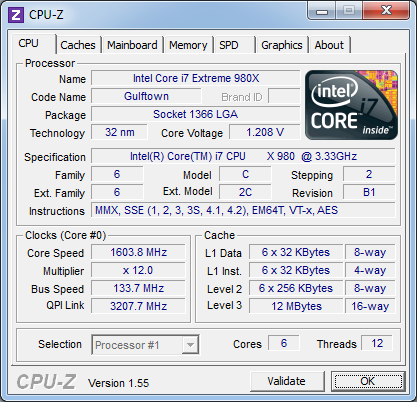
\includegraphics[scale=1]{imgs/cpu-z.png} 
\end{center}

%%%%%%%%%%%%%%%%%%%%%%%%%%%%%%%%%%%%%%%%%%%%%%%%%%%%%%%%%%%%%%%%

\newpage
\section{Трассировка лучей}
Классический ray tracing~[\cite{sivakov}], или метод трассировки лучей, предложен Артуром Аппелем (Arthur Appel) еще аж в 1968 году и дополнен алгоритмом общей рекурсии, разработанным Whitted в 1980 году. Понадобилось почти 12 лет эволюции вычислительных систем, прежде чем этот алгоритм стал доступен для широкого применения в практических приложениях. Реализация высокопроизводительной версии трассировки лучей уже предпринимаются различными компаниями. О сложности задачи трассировки лучей можно прочитать в соответствующих источниках~[\cite{biovulf}].

\subsection{Алгоритмы трассировки лучей}
Суть метода заключается в отслеживании траекторий лучей и расчета взаимодействий с лежащими на траекториях объектами, от момента испускания лучей источником света до момента попадания в камеру. Под взаимодействием луча с объектами понимаются процессы диффузного (в смысле модели локальной освещенности), многократного зеркального отражения от их поверхности и прохождение лучей сквозь прозрачные объекты. Таким образом, ray tracing – первый метод расчета глобального освещения, рассматривающий освещение, затенение (расчет тени), многократные отражения и преломления. Различают два основных вида метода трассировки лучей: \textbf{\textit{прямой}} -- \index{forward ray tracing}forward ray tracing, и \textbf{\textit{обратный}} -- \index{backward ray tracing}backward ray tracing.

\subsubsection{Прямой метод трассировки лучей}
В прямом методе траектории лучей строятся от источника ко всем точкам всех объектов сцены (первичные лучи). Затем проверяется ориентация каждой точки относительно источника, и, если она лежит на стороне объекта, обращенной в противоположную от источника сторону, точка из расчетов освещенности исключается. Для всех остальных точек вычисляется освещенность с помощью локальной модели освещения. Если объект не является отражающим или прозрачным, то есть поверхность объекта только диффузно рассеивает свет, траектория луча на этой точке обрывается (заканчивается). Если же поверхность объекта обладает свойством отражения (\index{reflection}reflection) и/или преломления (\index{refraction}refraction), из точки строятся новые лучи, направления которых совершенно точно определяются законами отражения и преломления.
\par
    Для построенных таким образом траекторий новых лучей может быть только три исхода. Луч либо выходит за пределы видимой из камеры области сцены, в этом случае все проделанные для него до этого момента расчеты освещенности отбрасываются, поскольку они не принимают участия в формировании изображения. Или луч попадает в камеру, тогда рассчитанная освещенность формирует цвет соответствующего пиксела изображения. Или луч встречает на своем пути новый
объект, тогда для новой точки пересечения повторяется расчет освещенности и построения лучей отражения и преломления в зависимости от свойств поверхности объекта (рекурсия). Построение новых траекторий и расчеты ведутся до тех пор, пока все лучи либо попадут в камеру, либо выйдут за пределы видимой области. Очевидно, что при прямой трассировке лучей мы вынуждены выполнять расчеты для лучей, которые не попадут в камеру, то есть, проделывать бесполезную работу. По некоторым оценочным данным доля таких "слепых"лучей довольно велика. Эта главная, хотя и далеко не единственная, причина того, что метод прямой трассировки лучей считается неэффективным и на практике не используется(в чистом виде).

\subsubsection{Обратный метод трассировки лучей}
Обратной метод трассировки лучей, или backward ray tracing. Этот метод расчетов основывается на построении лучей от наблюдателя через плоскость экрана вглубь сцены, а не от источника, то есть -- наоборот. Этот способ достаточно изящен, что позволяет решить массу проблем, возникающих при прямой трассировке, а сам метод отличается простотой и понятностью. Лучи теперь строятся иначе. А именно, по двум точкам: первая точка, общая для всех лучей – положение камеры (наблюдателя), вторая точка определяется положением пиксела на плоскости видового окна. Таким образом, направление каждого луча строго определено (две точки в пространстве определяют одну и только одну прямую – школьный курс геометрии), и количество первичных лучей также известно – это общее количество пикселей видового окна. Например, если видовое окно имеет 1920 пикселей по ширине и 1200 пикселей по высоте, количество лучей составит 1920 х 1200 = 2 304 000. Каждый луч
вдоль заданного направления продлевается от наблюдателя вглубь трехмерной сцены, и для каждой траектории выполняется проверка на пересечение со всеми объектами сцены и с отсекающими плоскостями. Если пересечений с объектами нет, а есть пересечение только с плоскостью отсечения, значит луч выходит за пределы видимой части сцены, и соответствующему пикселю видового окна присваивается цвет фона. Если луч пересекается с объектами сцены, то среди всех объектов выбирается тот, который ближе всего к наблюдателю. В точке пересечения с таким объектом строится три новых, так называемых вторичных луча. \par

\begin{center}
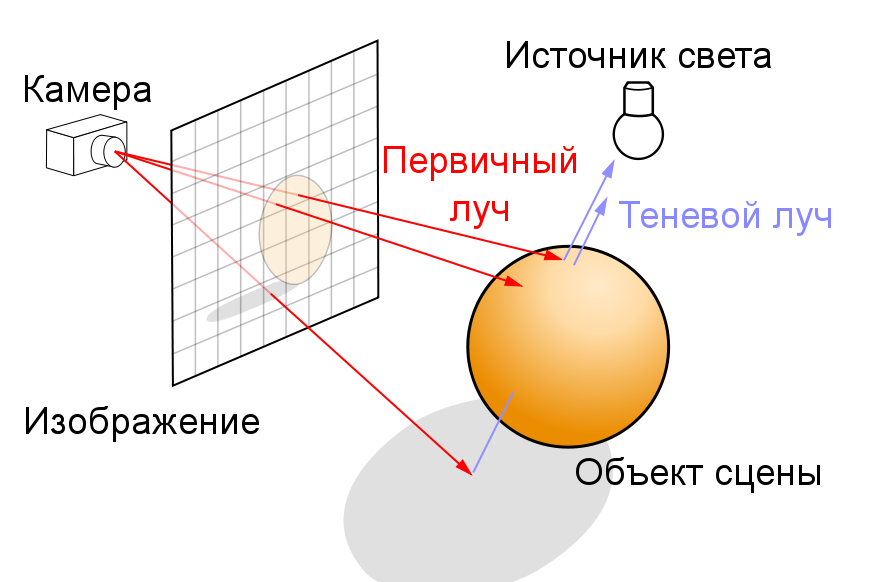
\includegraphics[scale=0.5]{imgs/Ray_trace_diagram_rus.png} 
\end{center}

Первый луч строится в направлении источника света. Если источников несколько, строится несколько таких лучей, по одному на каждый источник. Основное назначение этого луча – определить ориентацию точки (обращена точка к источнику или от него), наличие объектов, закрывающих точку от источника света, и расстояние до источника света. Если точка обращена в противоположную сторону от источника света или закрыта другим непрозрачным объектом, освещенность от такого источника не рассчитывается, точка находится в тени. В случае затеняющего прозрачного объекта интенсивность освещения уменьшается в соответствии со степенью прозрачности. Если точка закрыта от освещения всеми источниками сцены, ей присваивается фоновый (\index{ambient или фоновый цвет}ambient) цвет. В противном случае точка освещена, интенсивность и цвет освещения рассчитываются при помощи локальной модели освещенности, как сумма освещенностей от всех источников, для которых эта точка не закрыта другими объектами. Этот тип луча получил название \index{shadow ray или теневой луч} \textit{\textbf{shadow ray}} (иногда его еще называют \index{illumination ray}illumination ray) – теневой луч. Если поверхность объекта не является отражающей и непрозрачна, теневой луч – единственный тип лучей который строится, траектория первичного луча обрывается (заканчивается), и дальнейшие расчеты не выполняются. Рассчитанный цвет (освещенности или тени) присваивается тому пикселю видового окна, через который проходит соответствующий первичный луч.
   \par
   Второй луч строится, если поверхность объекта обладает отражающими свойствами, и называется \index{reflection ray или отраженный луч} reflection ray, или луч отражения. Направление отраженного луча определяется по закону:
$$
	\vec{R} = \vec{I} - 2 \cdot \vec{N} (\vec{N} , \vec{I})
$$
где $\vec{R}$ - отраженный луч, $\vec{I}$ - падающий первичный луч, $\vec{N}$ - нормаль к поверхности в точке соударения.
Для отраженного луча проверяется возможность пересечения с другими объектами сцены. Если пересечений нет, то интенсивность и цвет отраженного луча равна интенсивности и цвету фона. Если пересечение есть, то в новой точке снова строится три типа лучей – теневые, отражения и преломления.
Третий луч строится, если поверхность объекта прозрачна, и носит название \index{transparency ray или преломленный луч}transparency ray, т. е. луч преломленный. Направление для преломленного луча определяется следующим образом:
$$
 \vec{T} = \frac{n_1}{n_2} \cdot \vec{I} - \left[ \cos \alpha + \frac{n_1}{n_2} \cdot \left(\vec{N},\vec{I} \ \right) \right] \cdot \vec{N}
$$
$$
\cos \alpha = \sqrt{1 - \left( \frac{n_1}{n_2} \right) ^2 \cdot \left(1-\left(\vec{N},\vec{I}\ \right)^2\right)}
$$
где $\vec{T}$ - переломленный луч, $n_1$ - коэффициент рефракции для первой среды ( в которой растространяется первичный луч ), $n_2$ - коэффициент рефракции для второй среды прозрачного объекта.

Так же, как и в предыдущем случае, проверяется пересечение вновь построенного луча с объектами, и, если они есть, в новой точке строятся три луча, если нет -- используется интенсивность и цвет фона.

Таким образом, для каждого первичного луча можно построить древовидную структуру. Если древовидная структура для данного луча построена, то расчет освещенности можно выполнить в следующем порядке. Для каждой ветви дерева спускаемся вдоль древовидной структуры к последнему пересечению вторичного луча и поверхности (будем дальше называть их узлами). Поскольку это последний узел в цепи, то  вкладов от преломлений и отражений нет, поэтому, освещенность узла вычисляется при помощи локальной модели освещения с учетом видимости источников света для данного узла. Затем, вычисленная освещенность передается вверх по ветви к следующему ближайшему узлу. Освещенность в этом узле будет вычисляться по формуле:

$$
 \vec{I}_{total} = \vec{I}_{local} + K_{reflection} \cdot \vec{I}_{reflection} + K_{refraction} \cdot \vec{I}_{refraction}
$$

где $\vec{I}_{total}$ - полная освещенность в точке, $\vec{I}_{local}$ - локальная освещенность в точке, вычисленная от источников освещения с помощью одной из локальной модели освещенности, $K_{reflection}$ - коэффициент, определяющий отражающие свойства поверхности, $\vec{I}_{reflection}$ - освещенность предыдущей точки, переданная вдоль ветки отражения,   $K_{refraction}$ - коэффициент, определяющий преломляющие свойства поверхности $\vec{I}_{refraction}$ - освещенность предыдущей точки, переданная вдоль ветки преломления

Естественным завершением трассировки лучей является выход всех испущенных вторичных лучей за пределы видимой области и их рассеяние на чисто диффузных объектах. Результат вычислений будет наиболее точным. Но, если сцена достаточно сложна, такой расчет будет очень медленным, а в некоторых случаях и невозможным по причине ограниченности аппаратных ресурсов. Легко увидеть, что вклад освещенности от каждого нового вторичного луча очень быстро уменьшается по той простой причине, что коэффициенты свойств отражения и преломления материалов меньше единицы. Поэтому часто трассировку лучей прекращают, когда вклад от следующего узла ветви становится меньше заданной величины. Это также достаточно точный метод расчетов, который может быть использован для получения качественных результатов при определенных условиях. Наконец, для получения оценочного расчета можно оборвать трассировку лучей после выполнения заданного количества итераций, это самый быстрый и наименее точный расчет.

\subsubsection{Достоинства и недостатки}

Основные достоинства рекурсивного метода обратной трассировки лучей – расчет теней, многократных отражений и преломлений, значительно повысивших степень реалистичности получаемых изображений.
Основные недостатки: неучет вторичного освещения от диффузно отраженного объектами света; низкая скорость и высокая вычислительная стоимость расчетов – в классическом рейтресинге необходимо проверять на пересечение каждый луч со всеми объектами сцены, в результате от 70 до 95 процентов всего времени расчетов тратится на вычисление пересечений; резкие границы цветовых переходов тени/подсветок/прозрачности; \index{aliasing}aliasing – "зазубренность" линий и т. д.; дискретность определяющих цвет пиксела первичных лучей – одного первичного луча недостаточно для корректного определения цвета пиксела, формирующего изображение.


\subsection{Модели освещения}

В соответствии с принятым в компьютерной графике подходом, расчет освещенности распадается на две основные задачи. Первая – определить способ расчета освещенности в произвольной точке трехмерного пространства, решается при помощи построения обобщенной математической модели освещенности (Illuminating model). Вторая задача – применение Illuminating model для компьютерных расчетов освещенности трехмерных объектов с конкретной геометрией и свойствами поверхности, решается при помощи так называемой модели затенения (Shading model).

Моделей освещенности к настоящему моменту разработано несколько. Самая первая,и самая простая – локальная модель освещенности. Эта модель не рассматривает процессы светового взаимодействия объектов сцены между собой, а только расчет освещенности самих объектов. Вторая, глобальная модель освещенности – Global Illuminations, рассматривает трехмерную сцену как единую систему и пытается описывать освещение с учетом взаимного влияния объектов. В рамках этой модели рассматриваются такие вопросы, как многократное отражение и преломление света (ray tracing), рассеянное освещение (radiosity), каустик(caustic) и фотонные карты (photon mapping) и другие. 

\subsubsection{Глобальные модели освещения}

Глобальное освещение (global illumination) — это название ряда алгоритмов, используемых в 3D-графике, которые предназначены для добавления более реалистичного освещения в трёхмерные сцены. Такие алгоритмы учитывают не только свет, который поступает непосредственно от источника света (прямое освещение, англ. direct illumination), но и такие случаи, в которых лучи света от одного и того же источника, отражаются на других поверхностях сцены (непрямая освещенность, англ. indirect illumination).

Теоретически отражение, преломление, тень — примеры глобального освещения, потому что, для их имитации необходимо учитывать влияние одного объекта на другие (в отличие от случая когда на объект падает прямой свет). На практике, однако, только моделирование диффузного отражения или каустики называется глобальным освещением.

Изображения полученные в результате применения алгоритмов глобального освещения часто кажутся более фотореалистичными, чем те, в процессе рендеринга которых применялись алгоритмы только прямого освещения, но для просчета глобального освещения требуется гораздо больше времени.

\subsubsection{Локальные модели освещения}

Существующие локальные модели освещения можно разделить на две категории. К первой категории относятся эмпирические модели. Они обычно эффективны в плане быстродействия и некоторые из них дают довольно реалистичную картинку. Они обычно не оперируют такими физическими величинами, как световая энергия, или световой поток. Однако эти модели находят довольно широкое применение в областях, где не требуется точная физическая информация об освещении (например, спецэффекты в фильмах, программы для художников и дизайнеров, для рекламных целей)

Ко второй категории относятся модели, базирующиеся на физических представлениях о теории света. Изображения, полученные с использованием этих моделей, очень хорошо соотносятся с экспериментальными данными. Поэтому эти модели находят применение там, где важна точная имитация поведения света (оформление интерьеров, архитектура)

\subsubsection{Модель Фонга}

Это эмпирическая модель. В самом общем случае, в свете требования фотореалистичности, эта модель учитывает и неявное ambient-освещение. Ambient-освещение, или его еще называют фоновым (background), – это окружающее объект освещение от удаленных источников, чье положение и характеристики не известны. Необходимость учета ambient-освещения, пусть и очень грубо, обусловлена тем, что его вклад может быть достаточно велик – до 50\% от общей освещенности. В Local Illumination считают, что фоновое освещение задает цвет (и его интенсивность) объекта в отсутствии явных источников света или в тени. Не несет никакой информации об объекте, кроме значения простого цвета, равномерно заливающего контур объекта.

Интенсивность такого освещения постоянна и равномерно распределена во всем пространстве, расчет его отражения поверхностью выполняется по формуле:

$$
 \vec{I}_{amb} = K_{a} \cdot \vec{I}_{a}
$$

где $\vec{I}_{amb}$  - интенсивность отраженного ambient освещения, $K_{a}$ - коэффициент, характеризующий отражающие свойства поверхности для  ambient-освещения, $\vec{I}_{a}$ - исходная интенсивность ambient-света, падающего на поверхность.

Часть света от прямых источников зеркально отражается поверхностью, а остальной свет диффузно рассеивается во всех направлениях. Кроме чисто зеркального отражения, которое имеют идеально отполированные поверхности, различают так называемое glossiness или распределенное зеркальное отражение – отражение в некотором створе углов, а не на один единственный угол. Такое рассеяние света обусловлено микрорельефом ("шероховатостью") поверхности, то есть поверхность реальных объектов не является идеально гладкой, а состоит из большого количества микровыступов и впадин, которые зеркально отражают падающий свет под разными углами. Результатом glossy-отражения является specular highlight – яркий световой блик, имеющий размер в зависимости от степени шероховатости поверхности. 

Интенсивность рассеянного света зависит от угла падающего на поверхность света по закону Ламберта (Lambert):

$$
 \vec{I}_{diff} = K_{diff} \cdot \vec{I}_{d} \cdot \cos(\alpha)
$$
 
где $\vec{I}_{d}$ - интенсивность падающего на поверхность света, $K_{diff}$ - коэффициент, характеризующий рассеивающие свойства поверхности, $\cos(\alpha)$ - угол между направлением на источник света и нормалью поверхности

Другими словами, поверхность будет освещена больше, если свет падает на нее перпендикулярно ($\alpha = 0$), и меньше, если свет падает под любым другим углом, поскольку в этом случае увеличивается освещаемая площадь. Диффузно рассеянный свет является главным источником визуальной информации о геометрии трехмерных объектов.

Как было уже сказано ранее, свет отражается зеркально в некотором створе углов, и для большинства реальных материалов мы всегда видим зеркальную подсветку в форме светового пятна, а не в форме яркой точки. Поэтому, для расчета интенсивности зеркально отраженного света используется формула, предложенная Фонгом:

$$
 \vec{I}_{spec} = K_{spec} \cdot \vec{I}_{s} \cdot \cos^n(\beta)
$$

где $\vec{I}_{spec}$ - интенсивность зеркально отраженного света,  $\vec{I}_{s}$ - интенсивность источника света,  $\vec{K}_{s}$ - коэффициент, характеризующий свойства зеркального отражения поверхности
$\beta$ - угол между направлением идеального отражения и направлением на наблюдателя, степень $n$ определяет размер пятна светового блика, чем больше $n$, тем меньше световой блик, и тем ближе отражающие свойства поверхности к свойствам идеального зеркала.

Формула Фонга – пример компьютерной фикции, поскольку она не имеет физического смысла. Ее используют просто потому, что она дает хорошие практические результаты. 

Таким образом, локальная модель освещенности предполагает расчет отраженной фоновой освещенности, диффузного и зеркального отражения от прямых источников: 

$$
 \vec{I}_{local} =  K_{amb} \cdot \vec{I}_{amb} +  K_{diff} \cdot \vec{I}_{diff} \cdot \left( \vec{L},\vec{N} \right) + K_{spec} \cdot \vec{I}_{spec} \cdot \left( \vec{R},\vec{V} \right)^n
$$


\subsection{Модель камеры}

\subsubsection{Рассчет луча}

\subsubsection{Алгоритм антиалиасинга}

\subsection{Примитивы}
\subsubsection{\index{Плоскость}Плоскость}
Для определения пресечения луча с плоскостью, необходимо найти точку в пространстве, которая будет удовлетворять двум уравнениям: уравнению луча и уравнению плоскости.
\par
Уравнение луча:
\begin{equation}
\left\{
\begin{array}{ccccc}
x & = & x_p & + & t \cdot x_d \\
y & = & y_p & + & t \cdot y_d \\
z & = & z_p & + & t \cdot z_d \\
\end{array}
\right.
\label{equation_ray}
\end{equation}
или
$$
\vec{R}(t) = \vec{P} + t \cdot \vec{D}
$$
где $\vec{P} = \VECXYZ{p} $ - начало луча, а $\vec{D} = \VECXYZ{d} $ - направление луча. 
\par
Уравнение плоскости задается следующим образом:
\begin{equation}
Ax + By + Cz + D = 0
\label{equation_plane}
\end{equation}
\par
Для того, что бы найти точку пересечения луча с плоскостью, необходимо подставить уравнение (\ref{equation_ray}) в (\ref{equation_plane}):
$$
A(x_p + t \cdot x_d) + B(y_p + t \cdot y_d) + C(z_p + t \cdot z_d) + D = 0
$$
Раскроем скобки и привидём подобные
$$
t(Ax_d + By_d + Cz_d ) + Ax_p + By_p + Cz_p + D = 0
$$
выразим неизвестную величину t:
$$
 t = - \frac{Ax_p + By_p + Cz_p + D}{Ax_d + By_d + Cz_d}
$$
из уравнения видно, что луч либо пересекает плоскость в какой то точке, либо нет. Это связано с тем, что если $Ax_d + By_d + Cz_d = 0$, то плоскость и луч параллельны друг другу. Т.к. $\vec{N} = \VEC{A}{B}{C} $ - это нормаль к поверхности,а из геометрии известно, что если $( \vec{D} , \vec{P} ) = 0$, то вектора параллельны.
\par
   Для того, что бы найти величину $t$, необходимо рассчитать всего несколько скалярных произведений:
$$
t = - \frac{(\vec{P}, \vec{N}) + D}{(\vec{D}, \vec{N})}
$$
при условии, что $(\vec{D}, \vec{N}) \neq 0$
\begin{codebox}
\Procname{ $\proc{Алгоритм нахождения точки пересечения луча и плоскости}$}
\li \If $(\vec{D}, \vec{N}) \neq 0$
\li \Then $ t = - \displaystyle\frac{(\vec{P}, \vec{N}) + D}{(\vec{D}, \vec{N})} $
\li $point = \vec{P} + t \cdot \vec{D}$
\end{codebox}

\subsubsection{\index{Сфера}Сфера}
Для сферы необходимо проделать те же выкладки.
Уравнение сферы записывается следующем образом:
\begin{equation}
(x-x_c)^2 + (y-y_c)^2 + (z-z_c)^2 = r^2
\label{equation_sphere}
\end{equation}
где $\vec{C} = \VECXYZ{c}$ - центр сферы, а $r$ - радиус. Подставим уравнение (\ref{equation_ray}) в (\ref{equation_sphere}):
$$
\left( (x_0 + t \cdot x_d) - x_c \right)^2 + 
\left( (y_0 + t \cdot y_d) - y_c \right)^2 + 
\left( (z_0 + t \cdot z_d) - z_c \right)^2 = r^2
$$
раскроем скобки, приведем подобные
\begin{multline*}
(x_p + t \cdot x_d)^2 - 2(x_p + t \cdot x_d)\cdot x_c + x_c^2 + \\
 + (y_p + t \cdot y_d)^2 - 2(y_p + t \cdot y_d)\cdot y_c + y_c^2 + \\
 + (z_p + t \cdot z_d)^2 - 2(z_p + t \cdot z_d)\cdot z_c + z_c^2 = r^2
\end{multline*}
\begin{multline*}
x^2_p + 2x_px_d\cdot t + x_d^2 \cdot t^2 - 2 x_px_c - 2 x_dx_c \cdot t + x_c^2 + \\
 + y^2_p + 2y_py_d\cdot t + y_d^2 \cdot t^2 - 2 y_py_c - 2 y_dy_c \cdot t + y_c^2 + \\
 + z^2_p + 2z_pz_d\cdot t + z_d^2 \cdot t^2 - 2 z_pz_c - 2 z_dz_c \cdot t + z_c^2 = r^2
\end{multline*}

приведем уравнение в виду
\begin{equation}
a \cdot t^2 + b \cdot t + c = 0
\label{equation_square}
\end{equation}
после раскрытия скобок и приведения подобных, получаем:
\begin{eqnarray*}
\begin{split}
a &= x^2_d + y^2_d + z^2_d \\
b &= 2x_px_d + 2 y_py_d + 2z_pz_d - 2x_dx_c - 2y_dy_c - 2z_dz_c \\
c &= x_p^2 + y_p^2 + z_p^2 - 2x_px_c - 2y_py_c - 2z_pz_c + x_c^2 + y_c^2 + z_c^2 - r^2 \end{split}
\end{eqnarray*}
упростим
\begin{eqnarray*}
\begin{split}
a &= (\vec{D}, \vec{D}) \\
b &= 2x_d(x_0 - x_c) + 2y_d(y_0 - y_c) + 2z_d(z_0 - z_c) = 2 \cdot (\vec{D}, \vec{P}-\vec{C}) \\
c &= (x_0 - x_c)^2 + (y_0 - y_c)^2 + (z_0 - z_c)^2  - r^2 = 2 \cdot (\vec{P}-\vec{C},\vec{P}-\vec{C})
\end{split}
\end{eqnarray*}
перепишем в векторном виде
\begin{eqnarray*}
\begin{split}
a &= (\vec{D}, \vec{D}) \\
b &= 2 \cdot (\vec{D}, \vec{P}-\vec{C}) \\
c &= 2 \cdot (\vec{P}-\vec{C},\vec{P}-\vec{C}) - r^2
\end{split}
\end{eqnarray*}
Если уравнение (\ref{equation_square}) не имеет вещественных решений, то луч не пересекает сферу. Если имеется два решения, то наименьший положительный корень этого уравнения определит на луче ближайшую точку пересечения луча со сферой.
\par
Далее решаем обыкновенное квадратное уравнение, находим корни и получаем значение $t$,  при условие, что $a = (\vec{D},\vec{D}) \neq 0$
$$
t_{1,2} = \frac{-b \pm \sqrt{b^2 - 4 \cdot a \cdot c}}{2 \cdot a}
$$
\subsubsection{\index{Треугольник}Треугольник}
Алгоритм пересечения луча и треугольника основан на барицентрических координатах.
\par
Барицентрические координаты -- координаты точки $n$-мерного аффинного пространства $A^n$, отнесенные к некоторой фиксированной системе из $(n + 1)$-ой точки $p_0, p_1, \dots, p_n$ , не лежащих в $(n -1)$-мерном подпространстве. Пусть $z$ есть произвольная точка в $A^n$. Каждая точка $x \in A^n$ может быть единственным образом представлена в виде суммы
$$
	x = z + \alpha_1 \cdot z\vec{p_1} + \alpha_2 \cdot z\vec{p_2} + \cdots + \alpha_n \cdot z\vec{p_n} 
$$
где $\alpha_1, \alpha_2, \dots,  \alpha_n $ вещественные числа, удовлетворяющие условию
$$
\alpha_1 + \alpha_2 + \cdots + \alpha_n  = 1
$$
Числа $\alpha_1, \alpha_2, \dots,  \alpha_n $ называются барицентрическими координатами точки $x$. Легко видеть, что барицентрические координаты не зависят от выбора $z$.

Точка $T(u,v)$, принадлежащая треугольнику, может быть записана в виде:
\begin{equation}
\label{triangle_bar}
T(u,v) = (1-u-v)V_0 + uV_1 + vV_2
\end{equation}

\noindent где $(u,v)$ -- это бариецентрические координаты такие, что $u \geq 0$, $v \geq 0$ и $u + v \leq 1$

Вычисление пересечения между лучем(\ref{equation_ray}) и треугольником(\ref{triangle_bar}), это решение следующего уравнения:

$$
O + tD = (1-u-v)V_0 + uV_1 + vV_2
$$

\noindent после нескольких очевидных преобразований:

$$
O + tD = V_0 - uV_0 - vV_0 + uV_1 + vV_2
$$
$$
O - V_0 = - tD + uV_1 - uV_0 + vV_2 - vV_0
$$

$$
- tD + u(V_1 - V_0) + v(V_2 - V_0) = O - V_0
$$

\noindent получаем:

\begin{equation}
\label{ray_cross_tr}
\left[ -D, V_1 - V_0 , V_2 - V_0\right] 
\left[  
\begin{array}{c} t \\ u \\ v \\ \end{array}
\right] = O - V_0
\end{equation}

Что бы решить задачу, необходимо найти вектор $\VEC{t}{u}{v}$. Обозначив $E_1 = V_1 - V_0$, $E_2 = V_2 - V_0$ и $T = O - V_0$ решим уравнение (\ref{ray_cross_tr}), используя метод Крамера:

\begin{equation}
\label{ray_cross_tr_solv}
\left[  
\begin{array}{c} t \\ u \\ v \\ \end{array}
\right] = 
\frac{1}{| -D , E_1, E_2|} 
\left[  
	\begin{array}{lcccl}
	|& T , & E_1, &E_2 & | \\
	|&-D , & T  , &E_2 & | \\
	|&-D , & E_1, &T   & | \\
	\end{array}
\right] 
\end{equation}

\noindent Из курса линейной алгебры известно, что: $|A, B, C| = - (A \times C) \cdot B = - (C \times B) \cdot A$. Принимая во внимания этот факт, перепишем уравление (\ref{ray_cross_tr_solv}).

\begin{equation}
\label{ray_cross_tr_solv2}
\left[  
\begin{array}{c} t \\ u \\ v \\ \end{array}
\right] = 
\frac{1}{(D \times E_2)\cdot E_1} 
\left[  
	\begin{array}{c}
	(T \times E_1) \cdot E_2 \\
	(D \times E_2) \cdot T \\
	(T \times E_1) \cdot D \\
	\end{array}
\right] = 
\frac{1}{P \cdot E_1} 
\left[  
	\begin{array}{c}
	Q \cdot E_2 \\
	P \cdot T \\	
	Q \cdot D \\	
	\end{array}
\right]
\end{equation}
где $P = (D \times E_2)$ и $Q = T \times E_1$


%%%%%%%%%%%%%%%%%%%%%%%%%%%%%%%%%%%%%%%%%%%%%%%%%%%%%%%%%%%%%%%%%%%%%%%%%%%%%%%%%%%%%%%%%%%

\newpage
\section{Оптимизация}
Оптимизация -- как способ программирования по уровням архитектуры сверху вниз.

\subsection{Шаблоны C++}

\subsubsection{Понятие шаблона}

Шаблоны(Templates) были введены в язык C++ как средство, позволяющие параметризовать типы данных. Это связано с тем, что для классов или функций приходилось реализовывать одни и те же алгоритмы, но для разных типов данных. Получали дублирование кода, и тем самым росло число ошибок. 
Пример. Реализовать функцию, которая возвращает максимальное значение из 2 чисел.

\cppsource{src/deftemplate.tex}{Несколько реализация функции {\bf max}}

\noindent
и так далее. Приходится писать один и тот же код несколько раз. Во второй функции можно было допустить ошибку (например указать неправильный знак сравнения), которую потом очень трудно найти. Или наоборот, после обнаружения ошибки, придется править код во всех реализациях функции max (возможна ситуация, когда в нескольких местах ошибка была исправлена, а в остальных пропущена или забыта). С этими проблемами помогли справится шаблоны, которые параметризовали типы данных следующим образом:

\cppsource{src/definetemplate.tex}{Шаблонное определение функции {\bf max}}

%\noindent
Т. о. работу которую выполнял программист теперь выполняет компилятор. При вызове функции, в качестве параметров которых нужно сравнить два int, компилятор сам из шаблона выведет функцию max(int,int).
\subsubsection{Вычисление на шаблонах}
Сегодня шаблоны используют различным образом, не так как ожидали изобретатели
шаблонов С++. Сегодня программирование на шаблонах включают различные техники, такие как: обобщенное программирование, вычисление во время компиляции, шаблонные выражения(expression templates), мета-программирование, и др.

\noindent Рассмотрим пример вычисления факториала. \\
\noindent Факториал числа N это: $N! = N \cdot (N-1) \cdot \dots \cdot 1$

Рекурсивная реализация факториала, без использование шаблонов, приведена в следующем листинге:

\cppsource{src/rekfactorial.tex}{Рекурсивная реализация факториала}

Эту функцию следует использовать следующим образом:
\begin{verbatim}
cout << factorial(7) << endl;
\end{verbatim}
Вызывать рекурсивно функцию - это очень большие накладные расходы. Несмотря на то, что мы указало компилятору встроить функцию (inline), компилятор проигнорирует это, так как он не может сделать постановку в рекурсию. Можно добиться большего успеха, если реализовывать это, как класс с шаблоном.

\cppsource{src/templatefactorial.tex}{Реализация факториала на шаблонах}

Можно заметить, что у данного шаблона нет ни данных, ни функциональных участков, это только определение перечислимого типа. Для того чтобы можно было определить шаблон для n, нужно для начала определить шаблон для n-1, т. е. для n-2, n-3 и т. д. В итоге получаем рекурсию. Следует заметить, что в качестве параметра шаблона используется обычный тип int. По стандарту, в качестве параметров шаблона могут быть использованы только перечислимые типы. В нашем случае есть параметр шаблона типа int, это означает, что в этот шаблон будет подставлено постоянное число типа int. Что бы воспользоваться данным классом необходимо написать следующие:
\begin{verbatim}
cout << factorial<7>::ret << endl;
\end{verbatim}
Компилятор рекурсивно определяет значение факториала<7>, затем <6> и так далее. Так как это рекурсия, то что бы не зациклится необходимо вовремя остановится. Любая рекурсия нуждается в остановки, и это не исключение. Это можно сделать с помощью специализации шаблона(т.е. определение для частного случая).

\cppsource{src/specfactorial.tex}{Специализация шаблона вычисления факториала}

Когда компилятор начнет определять специализацию для <0>, то он подставит имеено эту реализацию и рекурсия завершится. В результате, получится следующая структура:

\cppsource{src/finfactorial.tex}{Развернутая структура вычисления факториала}

Как видно из примера, от структуры уже ничего ни осталось и при уровне оптимизации начиная с O1, компилятор подсчитает выражение и вместо:
\begin{verbatim}
cout << factorial<7>::ret << endl;
\end{verbatim}
Подставит, подсчитанное выражение:
\begin{verbatim}
cout << 5040 << endl;
\end{verbatim}
Проверить это можно дизассемблировав данный пример и увидеть в коде число 5040.

\subsection{SIMD инструкции}
Применение SIMD инструкций в классе vec4.
\subsubsection{Базовые операции в классе vec4}

\subsubsection{Скалярное произведение векторов}

\subsection{Ускоряющие структуры}

\subsubsection{Алгоритм построения BVH}

\subsubsection{Алгоритм траверса луча через BVH}

%%%%%%%%%%%%%%%%%%%%%%%%%%%%%%%%%%%%%%%%%%%%%%%%%%%%%%%%%%%%%%%%%%%%%%%%%%%%%%%%%%%%%%%%%%%

\newpage
\section{Постановка и результаты экспериментов}

Эксперименты проводилимь на 6 ядерном компьютере с процессором Intel Core i7 980x с частотой 3.33GHz, оперативной памятью 12 Гб, ОС - Calculate Linux 11.0 x64. 

Для сборки приложения с библиотекой tbb, необходимо, что бы компилятор поддерживал лямбда выражения из нового стандарта c++0x. На данный момент, этот стандарт поддерживает компилятор GCC 4.5.2

\subsection{Timer}
Для того, чтобы точно оценивать время работы каждого из алгоритмов, очень важно иметь такой инструмент как таймер, способный оценить время работы алгоритма. 
Проблема в том, что стандарные методы операционных систем не работают с нужной точностью. Когда идет речь о том, чтобы оценить время, который должен исполнятся очень много миллионов раз в секунду, важен каждый такт процессора и точность в миллисекунду и уж тем более в секундах просто неприемлема.

Для очень точной оценки времени работы алгоритмов, был специально написан высокоточный таймер на языке c++, с использованием ассемблера (AT\&T - синтаксиса).
Таймер выдает время в тактах процессора и включает в себя разные режимы подсчета времени.

\subsubsection{Алгоритм работы высокоточного таймера}

\cppsource{src/timer.tex}{Метод Start() и Stop() класса Timer}


\subsubsection{Эксперименты с высокоточным таймером}

\subsection{Вектора и Expression templates}

\subsection{Тестовая сцена}

\subsection{Эффективность расспаралеливания}

\subsection{TBB vs OpenMP}

\subsection{Влияние SIMD инструкций на скорость работы}

\subsection{Компилирование высокоуровнего кода в ассемблер}

Ассемблерные вставки, которые показывают что вычисление отражающего луча это одно SSE.

%%%%%%%%%%%%%%%%%%%%%%%%%%%%%%%%%%%%%%%%%%%%%%%%%%%%%%%%%%%%%%%%%%%%%%%%%%%%%%%%%%%%%%%%%%%

\newpage
\section*{Заключение}
\addcontentsline{toc}{section}{Заключение} 
Задача трассировки лучей является по настоящему трудным испытанием для центрального процессора. Несмотря на то, что процессор обладает хорошей производительностью на ядро, общей производительности ему не хватает. Несмотря на столь малые мощности, удалось реализовать достаточно быстрый алгоритм на центральном процессоре. Для большей производительности была разработана эффективная параллельная версия программы с использованием библиотеки TBB и
стандарта параллельного OpenMP. Благодаря использованию языка с++ и технику шаблонных выражений, удалось еще повысить производительность программы. Программа продемонстрировала хорошую производительность: используя всего лишь один процессор можно получать изображения в реальном времени.

%%%%%%%%%%%%%%%%%%%%%%%%%%%%%%%%%%%%%%%%%%%%%%%%%%%%%%%%%%%%%%%%%%%%%%%%%%%%%%%%%%%%%%%%%%%

\newpage
\begin{thebibliography}{99}
	\bibitem{morozov_kazan} Морозов А. С. Трассировка лучей в реальном времени на многоядерном процессоре. Высокопроизводительные параллельные вычисления на кластерных системах (HPC-2008). Материалы Восьмой Международной конференции-семинара. Казань, ноябрь 17-19, 2008. Труды конференции — Казань: Изд. КГТУ, 2008. - С. 241.
	\bibitem{morozov_microsoft} Морозов А. С. Высокопроизводительная реализация трассировки лучей с использованием Microsoft MPI. Технологии Microsoft в теории и практике программирования. Материалы конференции /Под ред. Проф. В.П. Гергеля. - Нижний Новгород: Изд-во Нижегородского госуниверситета, 2009. - 527 с.
	\bibitem{morozov_pavt} Морозов А. С. Сравнительный анализ алгоритма трассировки лучей на системах с общей и разделяемой памятью. Параллельные вычислительные технологии (ПаВТ’2009): Труды международной научной конференции (Нижний Новгород, 30 марта - 3 апреля 2009 г.). - Челябинск: Изд. ЮурГУ, 2009. - 839 с
	\bibitem{latex} Львовский С.М. Набор и верстка в системе \LaTeX. – 4-е изд., стереотипн. – М.: МЦНМО, 2006
	\bibitem{alloftex} Кнут, Дональд, Э. Все про \TeX. : Пер. с англ. --- М. : Издательский дом ''Вильямс'', 2003. --- 560 с. : ил. --- Парал. Тит. англ.
	\bibitem{inteloptimize} Гербер Р., Бик А., Смит К., Тиан К. Оптимизация ПО. Сборник рецептов. --- СПб.: Питер, 2010. --- 352 с.: ил. --- (Серия ''Библиотека программиста'').
	\bibitem{templatecpp} Вандевурд, Дэвид, Джосаттис, Николаи М. Шаблоны C++: справочник разработчика. : Пер. с англ. --- М. : Издательский дом ''Вильямс'', 2008. --- 544 с. : ил. --- парал. тит. англ.
	\bibitem{straustrupcpp} Б. Страуструп Язык программирования C++. Специальное издание / Пер. с англ. --- М.: ООО ''Бином-Пресс'', 2006. --- 1104 с.: ил.
	\bibitem{sivakov} Сиваков И. Как компьютер рассчитывает изображения. Технология программного рендеринга, 11.03.2004. \\ (\href{http://www.fcenter.ru/online.shtml?articles/hardware/videos/8749}{http://www.fcenter.ru/online.shtml?articles/hardware/videos/8749})
	\bibitem{biovulf} Дмитрий Мороз. "Беовульф": Создание фильма, 11.12.2007.\\ (\href{http://www.3dnews.ru/editorial/beowulf}{http://www.3dnews.ru/editorial/beowulf})
	\bibitem{intelintrinsic} Intel® C++ Intrinsics Reference \\ (\href{http://www.intel.com/products/processor/manuals/}{http://www.intel.com/products/processor/manuals/})
	\bibitem{intelmanual} Intel 64 and IA-32.Architectures Software Developer's Manual \\ (\href{http://www.intel.com/products/processor/manuals/}{http://www.intel.com/products/processor/manuals/})
	\bibitem{tbbtutor} Intel® Threading Building Blocks. Tutorial \\ (\href{http://www.threadingbuildingblocks.org/}{http://www.threadingbuildingblocks.org/})
	\bibitem{tbbmanual} Intel® Threading Building Blocks. Reference Manual \\ (\href{http://www.threadingbuildingblocks.org/}{http://www.threadingbuildingblocks.org/})
	\bibitem{cppexpressiontemplate} C++ Expression Templates An Introduction to the Principles of Expression Templates, 2003 \\ (\href{http://www.angelikalanger.com/Articles/Cuj/ExpressionTemplates/ExpressionTemplates.htm}{http://www.angelikalanger.com/.../ExpressionTemplates.htm})
	\bibitem{intelcore980x} Шесть ядер для десктопа: Intel Core i7-980X Extreme Edition, 07.04.2010 \\ (\href{http://www.fcenter.ru/online.shtml?articles/hardware/processors/28480}{http://www.fcenter.ru/online.shtml?articles/hardware/processors/28480})
	\bibitem{rdtscp} How to Benchmark Code Execution Times on Intel IA-32 and IA-64 Instruction Set Architectures. September 2010
\end{thebibliography}

\newpage
\documentclass[12pt, a4paper]{article}
\usepackage[utf8]{inputenc}
\usepackage[russian]{babel} 
\usepackage[T2A]{fontenc}
\usepackage[pdftex]{graphicx}
\usepackage{amstext}
\usepackage{textcomp}
\usepackage{multicol}
\usepackage{hyperref}
\usepackage{setspace}
\usepackage[usenames,dvipsnames]{color} % для source-highlight
\usepackage{indentfirst}

% меняем размеры страницы
\usepackage{geometry}
\geometry{left=2.5cm}
\geometry{right=2.0cm}
\geometry{top=1.5cm}
\geometry{bottom=2.5cm}

% шрифты
%\defaultfontfeatures{Scale=MatchLowercase}
%\setmainfont[SmallCapsFont={* Caps}]{Liberation Serif}
%\usepackage{xltxtra}
%\setmainfont[Mapping=tex-text]{Linux Libertine O}
%\setmonofont[SmallCapsFont={Courier New}]{Courier New}
%\fontsize{10}{10}


%\usepackage{courier}
%\setmainfont[Mapping=tex-text]{Courier}


% изменение межстрочного интервала
\def\heightline{1.2}
\linespread{\heightline} % 1.3 - это полуторный

%%%%%%%%%%%%%%%%%%%%%%%%%%%%%%%%%%%%%%%%%%%%%%%%
%%% добавляем точки в Оглавление

\renewcommand{\thesection}{\arabic{section}.} 
\renewcommand{\thesubsection}{\arabic{section}.\arabic{subsection}.} 
\renewcommand{\thesubsubsection}{\arabic{section}.\arabic{subsection}.\arabic{subsubsection}.} 

%%%%%%%%%%%%%%%%%%%%%%%%%%%%%%%%%%%%%%%%%%%%%%%%

% определим новые команды
\def\VEC#1#2#3{\left( \begin{array}{c} #1 \\ #2 \\ #3 \end{array} \right) }
\def\VECXYZ#1{\left( \begin{array}{c} x_#1 \\ y_#1 \\ z_#1 \end{array} \right) }

\newcommand{\HRule}{\noindent\rule{\linewidth}{0.45mm}}

\newcounter{sourcecode}
\setcounter{sourcecode}{1}
\newcommand*{\cppsource}[2]{\par{\HRule \small \tt \bf \noindent \ Листинг \arabic{sourcecode}. {\rm \small #2} \vspace{0.25cm}}%
\addtocounter{sourcecode}{1} \input{#1} \HRule}

\makeindex

\begin{document}

\begin{titlepage}
\begin{center}
{\large Федеральное агентство по образованию Российской Федерации\\
\vspace{0.25em}
Государственное образовательное учреждение\\высшего профессионального образования\\Нижегородский государственный университет им. Н.И. Лобачевского\\
\vspace{0.25em}
Факультет вычислительной математики и кибернетики\\
\vspace{0.25em}
Кафедра математического обеспечения ЭВМ\\
\vspace{3em}
Дипломная работа\\
}
\vspace{1em}
{\bf \huge
	\textsf{ Трассировка лучей в реальном времени на x64~архитектуре \\ } 
}
\end{center}
\vspace{0.5cm}
\begin{multicols}{2}
\large 
\noindent 
Работа допущена к защите \\
Заведующий кафедрой МО ЭВМ \\
д.ф.--м.н., проф. \\

\vspace*{1em}
{ \noindent
\hspace*{1.5cm}\hbox to 0cm{\raisebox{-1em}{\small Подпись}}\hspace{-1.5cm}{\hrulefill\ Стронгин Р. Г. }
}

\vspace*{1.0em}
{ \noindent
\hbox to 0cm{\raisebox{0.25em}{<<\ \ \ \ \ \  >>}}{\hrulefill\ 2011 г. }
}
\vbox to 5 cm{\ }
Исполнитель: \\
студент 2 курса магистратуры \\
факультета ВМК группы 86М1 \\

\vspace*{1em}
{ \noindent
\hspace*{1.5cm}\hbox to 0cm{\raisebox{-1em}{\small Подпись}}\hspace{-1.5cm}{\hrulefill\ Морозов А. С. }
}

\vspace*{1.0em}
{ \noindent
\hbox to 0cm{\raisebox{0.25em}{<<\ \ \ \ \ \  >>}}{\hrulefill\ 2011 г. }
}
\\
Научный руководитель: д. т. н., \\
профессор кафедры МО ЭВМ \\

\vspace*{1em}
{ \noindent
\hspace*{1.5cm}\hbox to 0cm{\raisebox{-1em}{\small Подпись}}\hspace{-1.5cm}{\hrulefill\ Турлапов В. Е. }
}

\vspace*{1.0em}
{ \noindent\newcommand{\z}{\textbf{Задача. }}
\hbox to 0cm{\raisebox{0.25em}{<<\ \ \ \ \ \  >>}}{\hrulefill\ 2011 г. }
}
\end{multicols}

\vfill 
\begin{center} 
{\rm \large Нижний Новгород \\ 2011 г.} 
\end {center} 
\end{titlepage} 

\tableofcontents

\newpage
\section*{Введение}
\addcontentsline{toc}{section}{Введение} 
В кино индустрии к современной компьютерной графике предъявляются серьезные требования физически корректного моделирования о освещения сцен, состоящая из множества примитивов с различными характеристиками взаимодействия со светом. Даже малейшие неточности, могут отбросить художественный или анимационный фильм в рубрику любительского кино, и при этом не принести ожидаемой прибыли. Особенные требования предъявляются именно к художественному фильму, т. к. используемые спец эффекты должны выглядеть настолько реалистично, что бы зритель не смог различить, где настоящий актер, а где рисованный двойник. Используя только физически правильные модели и алгоритмы можно обеспечить растущую потребность в более реалистичной трехмерной графике. \par
   С каждым новым фильмом, каждый из нас видит прогресс в компьютерной графике. Картинка становится все красочнее и правдоподобнее, но это все не дается просто так. Естественно, платить за это приходится высокой вычислительной трудоемкостью расчетов. Несомненно, что с каждым годом производительность вычислительной техники растет, но она сразу же «расходуются» на новые спецэффекты. Существует наблюдение, которое гласит, что время расчета одного кадра не изменяется. Среднее время расчета полного фильма 15 лет назад занимал около 10-12 месяцев, так и сегодня тратят столько же времени, хотя при этом, надо заметить, что производительность современных компьютеров в десятки, а то и в сотни раз превышает производительность компьютеров того времени. Со временем улучшается и требования к самому изображению. Если несколько лет
назад картинка с разрешением 1024х768 считалась излишеством в компьютерной графики, то уже сейчас это слишком мало и все считают де факто FullHD\footnote{ \index{FullHD}FullHD -- это разрешение экрана 1920х1080 пикселей} , хотя уже задумываются о еще лучшем качестве. В последний год компьютерная индустрия, дабы не потерять зрителя, начала использовать новые технологии — 3D, которая требует еще большей вычислительной мощности. \par
   Именно за последние несколько лет компьютеры стали по настоящему параллельными. Появились многоядерные процессоры. И именно по этому, что 15 лет назад было трудоемкой задачей рендеринга, то сейчас это можно получить почти в реальном времени при том же качестве результата.

\newpage 
\section{Постановка задачи}
Главной целью данной работы является разработка и исследование алгоритма трассировки лучей на архитектуре x64 с применением ускоряющей структуры. Для решения главной задачи, требуется решить ряд следующих подзадач:
\begin{itemize}
	\item Реализовать высокопроизводительный алгоритм трассировки лучей на центральном процессоре
	\item Реализация и исследование оптимизированной версии с использованием векторных расширений архитектуры x64
	\item Реализация и исследование специализированного класса векторов для алгоритма трассировки лучей основанного на технологии шаблонных выражений, с применением векторных оптимизаций  - \index{SIMD}SIMD\footnote{ Single Instruction, Multiple Data — Одна Инструкция, Много Данных } инструкции 
	\item Реализация параллельной версии алгоритма трассировки лучей с использованием OpenMP, TBB
	\item Сравнение параллельной версии алгоритма трассировки лучей с использованием библиотеки TBB и расширения языка OpenMP
	\item Реализация ускоряющей структуры
	\item Сравнение реализации алгоритма с использованием ускоряющей структуры и без нее
\end{itemize}
   В качестве основного языка программирования выбирается язык С++, а для отображения результатов — кроссплатформенная библиотека SDL. 
   
\newpage 
\section{Архитектура центрального процессора}
\subsection{Архитектура процессоров семейства x86}
Рассмотрим основные архитектурные особенности центрального процессора.
Одни из базовых понятий для производительности процессора:
\begin{itemize}
	\item Latency (Латентность команды) --- это число тактов, необходимое для завершения одной команды с момента готовности входных данных команды(выборки их из памяти) и начало ее выполнения
	\item Throughput (Пропускная способность команды) --- это число тактов ожидания, которое требуется процессору перед запуском на выполнение такой же команды
\end{itemize}   

\subsection{Архитектура процессоров семейства x64}
\subsubsection{Архитектура процессора Intel Core i7 980X}
\noindent{\bf\ttОбзор}\\
Intel Core i7 — семейство процессоров x86-64 Intel. Core i7 980X это процессор семейства Gulftown вышедшего в 2010 году. Основные характеристики представлены с помощью программы cpu-z:
\begin{center}
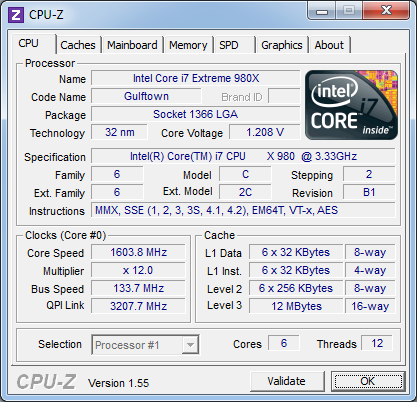
\includegraphics[scale=1]{imgs/cpu-z.png} 
\end{center}

%%%%%%%%%%%%%%%%%%%%%%%%%%%%%%%%%%%%%%%%%%%%%%%%%%%%%%%%%%%%%%%%

\newpage
\section{Трассировка лучей}
Классический ray tracing~[\cite{sivakov}], или метод трассировки лучей, предложен Артуром Аппелем (Arthur Appel) еще аж в 1968 году и дополнен алгоритмом общей рекурсии, разработанным Whitted в 1980 году. Понадобилось почти 12 лет эволюции вычислительных систем, прежде чем этот алгоритм стал доступен для широкого применения в практических приложениях. Реализация высокопроизводительной версии трассировки лучей уже предпринимаются различными компаниями. О сложности задачи трассировки лучей можно прочитать в соответствующих источниках~[\cite{biovulf}].

\subsection{Алгоритмы трассировки лучей}
Суть метода заключается в отслеживании траекторий лучей и расчета взаимодействий с лежащими на траекториях объектами, от момента испускания лучей источником света до момента попадания в камеру. Под взаимодействием луча с объектами понимаются процессы диффузного (в смысле модели локальной освещенности), многократного зеркального отражения от их поверхности и прохождение лучей сквозь прозрачные объекты. Таким образом, ray tracing – первый метод расчета глобального освещения, рассматривающий освещение, затенение (расчет тени), многократные отражения и преломления. Различают два основных вида метода трассировки лучей: \textbf{\textit{прямой}} -- \index{forward ray tracing}forward ray tracing, и \textbf{\textit{обратный}} -- \index{backward ray tracing}backward ray tracing.

\subsubsection{Прямой метод трассировки лучей}
В прямом методе траектории лучей строятся от источника ко всем точкам всех объектов сцены (первичные лучи). Затем проверяется ориентация каждой точки относительно источника, и, если она лежит на стороне объекта, обращенной в противоположную от источника сторону, точка из расчетов освещенности исключается. Для всех остальных точек вычисляется освещенность с помощью локальной модели освещения. Если объект не является отражающим или прозрачным, то есть поверхность объекта только диффузно рассеивает свет, траектория луча на этой точке обрывается (заканчивается). Если же поверхность объекта обладает свойством отражения (\index{reflection}reflection) и/или преломления (\index{refraction}refraction), из точки строятся новые лучи, направления которых совершенно точно определяются законами отражения и преломления.
\par
    Для построенных таким образом траекторий новых лучей может быть только три исхода. Луч либо выходит за пределы видимой из камеры области сцены, в этом случае все проделанные для него до этого момента расчеты освещенности отбрасываются, поскольку они не принимают участия в формировании изображения. Или луч попадает в камеру, тогда рассчитанная освещенность формирует цвет соответствующего пиксела изображения. Или луч встречает на своем пути новый
объект, тогда для новой точки пересечения повторяется расчет освещенности и построения лучей отражения и преломления в зависимости от свойств поверхности объекта (рекурсия). Построение новых траекторий и расчеты ведутся до тех пор, пока все лучи либо попадут в камеру, либо выйдут за пределы видимой области. Очевидно, что при прямой трассировке лучей мы вынуждены выполнять расчеты для лучей, которые не попадут в камеру, то есть, проделывать бесполезную работу. По некоторым оценочным данным доля таких "слепых"лучей довольно велика. Эта главная, хотя и далеко не единственная, причина того, что метод прямой трассировки лучей считается неэффективным и на практике не используется(в чистом виде).

\subsubsection{Обратный метод трассировки лучей}
Обратной метод трассировки лучей, или backward ray tracing. Этот метод расчетов основывается на построении лучей от наблюдателя через плоскость экрана вглубь сцены, а не от источника, то есть -- наоборот. Этот способ достаточно изящен, что позволяет решить массу проблем, возникающих при прямой трассировке, а сам метод отличается простотой и понятностью. Лучи теперь строятся иначе. А именно, по двум точкам: первая точка, общая для всех лучей – положение камеры (наблюдателя), вторая точка определяется положением пиксела на плоскости видового окна. Таким образом, направление каждого луча строго определено (две точки в пространстве определяют одну и только одну прямую – школьный курс геометрии), и количество первичных лучей также известно – это общее количество пикселей видового окна. Например, если видовое окно имеет 1920 пикселей по ширине и 1200 пикселей по высоте, количество лучей составит 1920 х 1200 = 2 304 000. Каждый луч
вдоль заданного направления продлевается от наблюдателя вглубь трехмерной сцены, и для каждой траектории выполняется проверка на пересечение со всеми объектами сцены и с отсекающими плоскостями. Если пересечений с объектами нет, а есть пересечение только с плоскостью отсечения, значит луч выходит за пределы видимой части сцены, и соответствующему пикселю видового окна присваивается цвет фона. Если луч пересекается с объектами сцены, то среди всех объектов выбирается тот, который ближе всего к наблюдателю. В точке пересечения с таким объектом строится три новых, так называемых вторичных луча. \par

\begin{center}
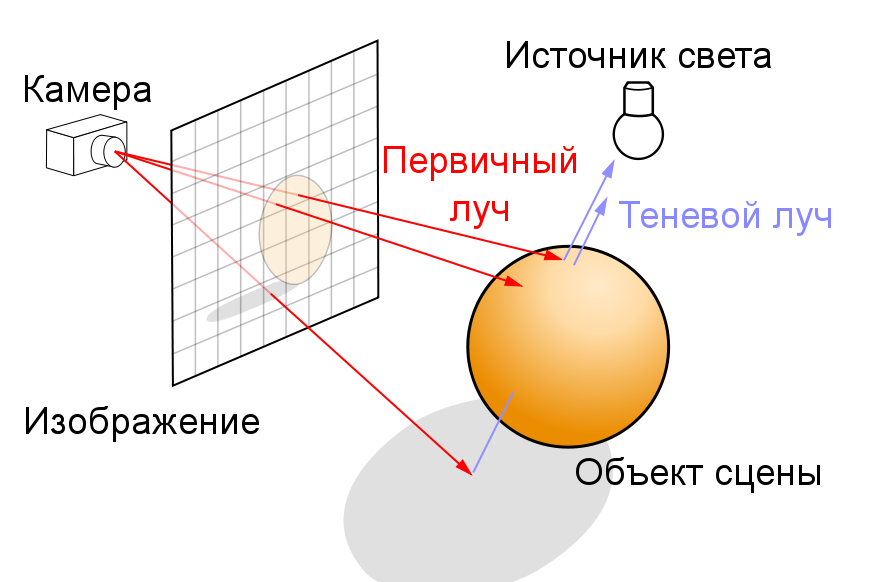
\includegraphics[scale=0.5]{imgs/Ray_trace_diagram_rus.png} 
\end{center}

Первый луч строится в направлении источника света. Если источников несколько, строится несколько таких лучей, по одному на каждый источник. Основное назначение этого луча – определить ориентацию точки (обращена точка к источнику или от него), наличие объектов, закрывающих точку от источника света, и расстояние до источника света. Если точка обращена в противоположную сторону от источника света или закрыта другим непрозрачным объектом, освещенность от такого источника не рассчитывается, точка находится в тени. В случае затеняющего прозрачного объекта интенсивность освещения уменьшается в соответствии со степенью прозрачности. Если точка закрыта от освещения всеми источниками сцены, ей присваивается фоновый (\index{ambient или фоновый цвет}ambient) цвет. В противном случае точка освещена, интенсивность и цвет освещения рассчитываются при помощи локальной модели освещенности, как сумма освещенностей от всех источников, для которых эта точка не закрыта другими объектами. Этот тип луча получил название \index{shadow ray или теневой луч} \textit{\textbf{shadow ray}} (иногда его еще называют \index{illumination ray}illumination ray) – теневой луч. Если поверхность объекта не является отражающей и непрозрачна, теневой луч – единственный тип лучей который строится, траектория первичного луча обрывается (заканчивается), и дальнейшие расчеты не выполняются. Рассчитанный цвет (освещенности или тени) присваивается тому пикселю видового окна, через который проходит соответствующий первичный луч.
   \par
   Второй луч строится, если поверхность объекта обладает отражающими свойствами, и называется \index{reflection ray или отраженный луч} reflection ray, или луч отражения. Направление отраженного луча определяется по закону:
$$
	\vec{R} = \vec{I} - 2 \cdot \vec{N} (\vec{N} , \vec{I})
$$
где $\vec{R}$ - отраженный луч, $\vec{I}$ - падающий пераичный луч, $\vec{N}$ - нормаль к поверхности в точке соударения.
Для отраженного луча проверяется возможность пересечения с другими объектами сцены. Если пересечений нет, то интенсивность и цвет отраженного луча равна интенсивности и цвету фона. Если пересечение есть, то в новой точке снова строится три типа лучей – теневые, отражения и преломления.
Третий луч строится, если поверхность объекта прозрачна, и носит название \index{transparency ray или преломленный луч}transparency ray, т. е. луч преломленный. Направление для преломленного луча определяется следующим образом:
$$
 \vec{T} = \frac{n_1}{n_2} \cdot \vec{I} - \left[ \cos \alpha + \frac{n_1}{n_2} \cdot \left(\vec{N},\vec{I} \ \right) \right] \cdot \vec{N}
$$
$$
\cos \alpha = \sqrt{1 - \left( \frac{n_1}{n_2} \right) ^2 \cdot \left(1-\left(\vec{N},\vec{I}\ \right)^2\right)}
$$
где $\vec{T}$ - переломленный луч, $n_1$ - коэффициент рефракции для первой среды ( в которой растространяется первичный луч ), $n_2$ - коэффициент рефракции для второй среды прозрачного объекта.

Так же, как и в предыдущем случае, проверяется пересечение вновь построенного луча с объектами, и, если они есть, в новой точке строятся три луча, если нет -- используется интенсивность и цвет фона.

Таким образом, для каждого первичного луча можно построить древовидную структуру. Если древовидная структура для данного луча построена, то расчет освещенности можно выполнить в следующем порядке. Для каждой ветви дерева спускаемся вдоль древовидной структуры к последнему пересечению вторичного луча и поверхности (будем дальше называть их узлами). Поскольку это последний узел в цепи, то  вкладов от преломлений и отражений нет, поэтому, освещенность узла вычисляется при помощи локальной модели освещения с учетом видимости источников света для данного узла. Затем, вычисленная освещенность передается вверх по ветви к следующему ближайшему узлу. Освещенность в этом узле будет вычисляться по формуле:

$$
 \vec{I}_{total} = \vec{I}_{local} + K_{reflection} \cdot \vec{I}_{reflection} + K_{refraction} \cdot \vec{I}_{refraction}
$$

где $\vec{I}_{total}$ - полная освещенность в точке, $\vec{I}_{local}$ - локальная освещенность в точке, вычисленная от источников освещения с помощью одной из локальной модели освещенности, $K_{reflection}$ - коэффициент, определяющий отражающие свойства поверхности, $\vec{I}_{reflection}$ - освещенность предыдущей точки, переданная вдоль ветки отражения,   $K_{refraction}$ - коэффициент, определяющий преломляющие свойства поверхности $\vec{I}_{refraction}$ - освещенность предыдущей точки, переданная вдоль ветки преломления

Естественным завершением трассировки лучей является выход всех испущенных вторичных лучей за пределы видимой области и их рассеяние на чисто диффузных объектах. Результат вычислений будет наиболее точным. Но, если сцена достаточно сложна, такой расчет будет очень медленным, а в некоторых случаях и невозможным по причине ограниченности аппаратных ресурсов. Легко увидеть, что вклад освещенности от каждого нового вторичного луча очень быстро уменьшается по той простой причине, что коэффициенты свойств отражения и преломления материалов меньше единицы. Поэтому часто трассировку лучей прекращают, когда вклад от следующего узла ветви становится меньше заданной величины. Это также достаточно точный метод расчетов, который может быть использован для получения качественных результатов при определенных условиях. Наконец, для получения оценочного расчета можно оборвать трассировку лучей после выполнения заданного количества итераций, это самый быстрый и наименее точный расчет.

\subsubsection{Достоинства и недостатки}

Основные достоинства рекурсивного метода обратной трассировки лучей – расчет теней, многократных отражений и преломлений, значительно повысивших степень реалистичности получаемых изображений.
Основные недостатки: неучет вторичного освещения от диффузно отраженного объектами света; низкая скорость и высокая вычислительная стоимость расчетов – в классическом рейтресинге необходимо проверять на пересечение каждый луч со всеми объектами сцены, в результате от 70 до 95 процентов всего времени расчетов тратится на вычисление пересечений; резкие границы цветовых переходов тени/подсветок/прозрачности; \index{aliasing}aliasing – "зазубренность" линий и т. д.; дискретность определяющих цвет пиксела первичных лучей – одного первичного луча недостаточно для корректного определения цвета пиксела, формирующего изображение.


\subsection{Модели освещения}

В соответствии с принятым в компьютерной графике подходом, расчет освещенности распадается на две основные задачи. Первая – определить способ расчета освещенности в произвольной точке трехмерного пространства, решается при помощи построения обобщенной математической модели освещенности (Illuminating model). Вторая задача – применение Illuminating model для компьютерных расчетов освещенности трехмерных объектов с конкретной геометрией и свойствами поверхности, решается при помощи так называемой модели затенения (Shading model).

Моделей освещенности к настоящему моменту разработано несколько. Самая первая,и самая простая – локальная модель освещенности. Эта модель не рассматривает процессы светового взаимодействия объектов сцены между собой, а только расчет освещенности самих объектов. Вторая, глобальная модель освещенности – Global Illuminations, рассматривает трехмерную сцену как единую систему и пытается описывать освещение с учетом взаимного влияния объектов. В рамках этой модели рассматриваются такие вопросы, как многократное отражение и преломление света (ray tracing), рассеянное освещение (radiosity), каустик(caustic) и фотонные карты (photon mapping) и другие. 

\subsubsection{Глобальные модели освещения}

Глобальное освещение (global illumination) — это название ряда алгоритмов, используемых в 3D-графике, которые предназначены для добавления более реалистичного освещения в трёхмерные сцены. Такие алгоритмы учитывают не только свет, который поступает непосредственно от источника света (прямое освещение, англ. direct illumination), но и такие случаи, в которых лучи света от одного и того же источника, отражаются на других поверхностях сцены (непрямая освещенность, англ. indirect illumination).

Теоретически отражение, преломление, тень — примеры глобального освещения, потому что, для их имитации необходимо учитывать влияние одного объекта на другие (в отличие от случая когда на объект падает прямой свет). На практике, однако, только моделирование диффузного отражения или каустики называется глобальным освещением.

Изображения полученные в результате применения алгоритмов глобального освещения часто кажутся более фотореалистичными, чем те, в процессе рендеринга которых применялись алгоритмы только прямого освещения, но для просчета глобального освещения требуется гораздо больше времени.

\subsubsection{Локальные модели освещения}

Существующие локальные модели освещения можно разделить на две категории. К первой категории относятся эмпирические модели. Они обычно эффективны в плане быстродействия и некоторые из них дают довольно реалистичную картинку. Они обычно не оперируют такими физическими величинами, как световая энергия, или световой поток. Однако эти модели находят довольно широкое применение в областях, где не требуется точная физическая информация об освещении (например, спецэффекты в фильмах, программы для художников и дизайнеров, для рекламных целей)

Ко второй категории относятся модели, базирующиеся на физических представлениях о теории света. Изображения, полученные с использованием этих моделей, очень хорошо соотносятся с экспериментальными данными. Поэтому эти модели находят применение там, где важна точная имитация поведения света (оформление интерьеров, архитектура)

\subsubsection{Модель Фонга}

Это эмпирическая модель. В самом общем случае, в свете требования фотореалистичности, эта модель учитывает и неявное ambient-освещение. Ambient-освещение, или его еще называют фоновым (background), – это окружающее объект освещение от удаленных источников, чье положение и характеристики не известны. Необходимость учета ambient-освещения, пусть и очень грубо, обусловлена тем, что его вклад может быть достаточно велик – до 50\% от общей освещенности. В Local Illumination считают, что фоновое освещение задает цвет (и его интенсивность) объекта в отсутствии явных источников света или в тени. Не несет никакой информации об объекте, кроме значения простого цвета, равномерно заливающего контур объекта.

Интенсивность такого освещения постоянна и равномерно распределена во всем пространстве, расчет его отражения поверхностью выполняется по формуле:

$$
 \vec{I}_{amb} = K_{a} \cdot \vec{I}_{a}
$$

где $\vec{I}_{amb}$  - интенсивность отраженного ambient освещения, $K_{a}$ - коэффициент, характеризующий отражающие свойства поверхности для  ambient-освещения, $\vec{I}_{a}$ - исходная интенсивность ambient-света, падающего на поверхность.

Часть света от прямых источников зеркально отражается поверхностью, а остальной свет диффузно рассеивается во всех направлениях. Кроме чисто зеркального отражения, которое имеют идеально отполированные поверхности, различают так называемое glossiness или распределенное зеркальное отражение – отражение в некотором створе углов, а не на один единственный угол. Такое рассеяние света обусловлено микрорельефом ("шероховатостью") поверхности, то есть поверхность реальных объектов не является идеально гладкой, а состоит из большого количества микровыступов и впадин, которые зеркально отражают падающий свет под разными углами. Результатом glossy-отражения является specular highlight – яркий световой блик, имеющий размер в зависимости от степени шероховатости поверхности. 

Интенсивность рассеянного света зависит от угла падающего на поверхность света по закону Ламберта (Lambert):

$$
 \vec{I}_{diff} = K_{diff} \cdot \vec{I}_{d} \cdot \cos(\alpha)
$$
 
где $\vec{I}_{d}$ - интенсивность падающего на поверхность света, $K_{diff}$ - коэффициент, характеризующий рассеивающие свойства поверхности, $\cos(\alpha)$ - угол между направлением на источник света и нормалью поверхности

Другими словами, поверхность будет освещена больше, если свет падает на нее перпендикулярно ($\alpha = 0$), и меньше, если свет падает под любым другим углом, поскольку в этом случае увеличивается освещаемая площадь. Диффузно рассеянный свет является главным источником визуальной информации о геометрии трехмерных объектов.

Как было уже сказано ранее, свет отражается зеркально в некотором створе углов, и для большинства реальных материалов мы всегда видим зеркальную подсветку в форме светового пятна, а не в форме яркой точки. Поэтому, для расчета интенсивности зеркально отраженного света используется формула, предложенная Фонгом:

$$
 \vec{I}_{spec} = K_{spec} \cdot \vec{I}_{s} \cdot \cos^n(\beta)
$$

где $\vec{I}_{spec}$ - интенсивность зеркально отраженного света,  $\vec{I}_{s}$ - интенсивность источника света,  $\vec{K}_{s}$ - коэффициент, характеризующий свойства зеркального отражения поверхности
$\beta$ - угол между направлением идеального отражения и направлением на наблюдателя, степень $n$ определяет размер пятна светового блика, чем больше $n$, тем меньше световой блик, и тем ближе отражающие свойства поверхности к свойствам идеального зеркала.

Формула Фонга – пример компьютерной фикции, поскольку она не имеет физического смысла. Ее используют просто потому, что она дает хорошие практические результаты. 

Таким образом, локальная модель освещенности предполагает расчет отраженной фоновой освещенности, диффузного и зеркального отражения от прямых источников: 

$$
 \vec{I}_{local} =  K_{amb} \cdot \vec{I}_{amb} +  K_{diff} \cdot \vec{I}_{diff} \cdot \left( \vec{L},\vec{N} \right) + K_{spec} \cdot \vec{I}_{spec} \cdot \left( \vec{R},\vec{V} \right)^n
$$



\subsection{Примитивы}
\subsubsection{\index{Плоскость}Плоскость}
Для определения пресечения луча с плоскостью, необходимо найти точку в пространстве, которая будет удовлетворять двум уравнениям: уравнению луча и уравнению плоскости.
\par
Уравнение луча:
\begin{equation}
\left\{
\begin{array}{ccccc}
x & = & x_0 & + & t \cdot x_d \\
y & = & y_0 & + & t \cdot y_d \\
z & = & z_0 & + & t \cdot z_d \\
\end{array}
\right.
\label{equation_ray}
\end{equation}
или
$$
\vec{R}(t) = \vec{O} + t \cdot \vec{D}
$$
где $O = \VECXYZ{0} $ - начало луча, а $D = \VECXYZ{d} $ - направление луча. 
\par
Уравнение плоскости задается следующим образом:
\begin{equation}
Ax + By + Cz + D = 0
\label{equation_plane}
\end{equation}
\par
Для того, что бы найти точку пересечения луча с плоскостью, необходимо подставить уравнение (\ref{equation_ray}) в (\ref{equation_plane}):
$$
A(x_0 + t \cdot x_d) + B(y_0 + t \cdot y_d) + C(z_0 + t \cdot z_d) + D = 0
$$
Раскроем скобки и приведем подобные
$$
t(Ax_d + By_d + Cz_d ) + Ax_0 + By_0 + Cz_0 + D = 0
$$
найдем неизвестную величину t
$$
 t = - \frac{Ax_0 + By_0 + Cz_0 + D}{Ax_d + By_d + Cz_d}
$$
из уравнения видно, что луч либо пересекает плоскость в какой то точке, либо нет. Это связано с тем, что если $Ax_d + By_d + Cz_d = 0$, то плоскость и луч параллельны друг другу. Т.к. $P = \VEC{A}{B}{C} $ - это нормаль к поверхности, то из геометрии известно, что если $( D , P ) = 0$, то вектора параллельны.
\par
   Для того, что бы найти величину $t$, необходимо рассчитать всего несколько скалярных произведений:
$$
t = - \frac{(O, P) + D}{(D, P)}
$$
при условии, что $(D, P) \neq 0$

\subsubsection{\index{Сфера}Сфера}
Для сферы необходимо проделать те же выкладки.
Уравнение луча:
\begin{equation}
\left\{
\begin{array}{ccccc}
x & = & x_0 & + & t \cdot x_d \\
y & = & y_0 & + & t \cdot y_d \\
z & = & z_0 & + & t \cdot z_d \\
\end{array}
\right.
\label{equation_ray}
\end{equation}
или
$$
\vec{R}(t) = \vec{O} + t \cdot \vec{D}
$$
Уравнение сферы записывается следующем образом:
\begin{equation}
(x-x_c)^2 + (y-y_c)^2 + (z-z_c)^2 = r^2
\label{equation_sphere}
\end{equation}
где $S = \VECXYZ{c}$ - центр сферы, а $r$ - радиус. Подставим уравнение (\ref{equation_ray}) в (\ref{equation_sphere}):
$$
\left( (x_0 + t \cdot x_d) - x_c \right)^2 + 
\left( (y_0 + t \cdot y_d) - y_c \right)^2 + 
\left( (z_0 + t \cdot z_d) - z_c \right)^2 = r^2
$$
приведем это уравнение в виду
\begin{equation}
A \cdot t^2 + B \cdot t + C = 0
\label{equation_square}
\end{equation}
после раскрытия скобок и приведения подобных, получаем:
\par
$$
A = x^2_d + y^2_d + z^2_d
$$ 
\par
$$
B = 2x_d(x_0 - x_c) + 2y_d(y_0 - y_c)  + 2z_d(z_0 - z_c) 
$$ 
\par
$$
C = (x_0 - x_c)^2 + (y_0 - y_c)^2 + (z_0 - z_c)^2 
$$
Если уравнение (\ref{equation_square}) не имеет вещественных решений, то луч не пересекает сферу. Если имеется два решения, то наименьший положительный корень этого уравнения определит на луче ближайшую точку пересечения луча со сферой.
\par
Рассмотрим подробнее как вычисляются коэффициенты $A$, $B$, $C$:
\par
$$
A = x^2_d + y^2_d + z^2_d = (D, D)
$$ 
\par
$$
B = 2x_d(x_0 - x_c) + 2y_d(y_0 - y_c)  + 2z_d(z_0 - z_c)  = 2 \cdot (D, D - S)
$$ 
\par
$$
C = (x_0 - x_c)^2 + (y_0 - y_c)^2 + (z_0 - z_c)^2 = (O - S, O - S )
$$
Далее решаем обыкновенное квадратное уравнение и находим корни и получаем значение $t$
$$
t_{1,2} = \frac{-B \pm \sqrt{B^2 - 4 \cdot A \cdot C}}{2 \cdot A}
$$

$$
t_{1} = \frac{ - 2 \cdot (\vec{D}, \vec{D} - \vec{S}) + \sqrt{(2 \cdot (\vec{D}, \vec{D} - \vec{S}))^2 - 4 \cdot (\vec{D}, \vec{D}) \cdot (\vec{O} - \vec{S}, \vec{O} - \vec{S} )}}{2 \cdot (\vec{D}, \vec{D})}
$$

$$
t_{2} = \frac{ - 2 \cdot (\vec{D}, \vec{D} - \vec{S}) - \sqrt{(2 \cdot (\vec{D}, \vec{D} - \vec{S}))^2 - 4 \cdot (\vec{D}, \vec{D}) \cdot (\vec{O} - \vec{S}, \vec{O} - \vec{S} )}}{2 \cdot (\vec{D}, \vec{D})}
$$

\subsubsection{\index{Треугольник}Треугольник}
Алгоритм пересечения луча и треугольника основан на барицентрических координатах.
\par
Барицентрические координаты -- координаты точки $n$-мерного аффинного пространства $A^n$, отнесенные к некоторой фиксированной системе из $(n + 1)$-ой точки $p_0, p_1, \dots, p_n$ , не лежащих в $(n -1)$-мерном подпространстве. Пусть $z$ есть произвольная точка в $A^n$. Каждая точка $x \in A^n$ может быть единственным образом представлена в виде суммы
$$
	x = z + \alpha_1 \cdot z\vec{p_1} + \alpha_2 \cdot z\vec{p_2} + \cdots + \alpha_n \cdot z\vec{p_n} 
$$
где $\alpha_1, \alpha_2, \dots,  \alpha_n $ вещественные числа, удовлетворяющие условию
$$
\alpha_1 + \alpha_2 + \cdots + \alpha_n  = 1
$$
Числа $\alpha_1, \alpha_2, \dots,  \alpha_n $ называются барицентрическими координатами точки $x$. Легко видеть, что барицентрические координаты не зависят от выбора $z$.

Точка $T(u,v)$, принадлежащая треугольнику, может быть записана в виде:
\begin{equation}
\label{triangle_bar}
T(u,v) = (1-u-v)V_0 + uV_1 + vV_2
\end{equation}

\noindent где $(u,v)$ -- это бариецентрические координаты такие, что $u \geq 0$, $v \geq 0$ и $u + v \leq 1$

Вычисление пересечения между лучем(\ref{equation_ray}) и треугольником(\ref{triangle_bar}), это решение следующего уравнения:

$$
O + tD = (1-u-v)V_0 + uV_1 + vV_2
$$

\noindent после нескольких очевидных преобразований:

$$
O + tD = V_0 - uV_0 - vV_0 + uV_1 + vV_2
$$
$$
O - V_0 = - tD + uV_1 - uV_0 + vV_2 - vV_0
$$

$$
- tD + u(V_1 - V_0) + v(V_2 - V_0) = O - V_0
$$

\noindent получаем:

\begin{equation}
\label{ray_cross_tr}
\left[ -D, V_1 - V_0 , V_2 - V_0\right] 
\left[  
\begin{array}{c} t \\ u \\ v \\ \end{array}
\right] = O - V_0
\end{equation}

Что бы решить задачу, необходимо найти вектор $\VEC{t}{u}{v}$. Обозначив $E_1 = V_1 - V_0$, $E_2 = V_2 - V_0$ и $T = O - V_0$ решим уравнение (\ref{ray_cross_tr}), используя метод Крамера:

\begin{equation}
\label{ray_cross_tr_solv}
\left[  
\begin{array}{c} t \\ u \\ v \\ \end{array}
\right] = 
\frac{1}{| -D , E_1, E_2|} 
\left[  
	\begin{array}{lcccl}
	|& T , & E_1, &E_2 & | \\
	|&-D , & T  , &E_2 & | \\
	|&-D , & E_1, &T   & | \\
	\end{array}
\right] 
\end{equation}

\noindent Из курса линейной алгебры известно, что: $|A, B, C| = - (A \times C) \cdot B = - (C \times B) \cdot A$. Принимая во внимания этот факт, перепишем уравление (\ref{ray_cross_tr_solv}).

\begin{equation}
\label{ray_cross_tr_solv2}
\left[  
\begin{array}{c} t \\ u \\ v \\ \end{array}
\right] = 
\frac{1}{(D \times E_2)\cdot E_1} 
\left[  
	\begin{array}{c}
	(T \times E_1) \cdot E_2 \\
	(D \times E_2) \cdot T \\
	(T \times E_1) \cdot D \\
	\end{array}
\right] = 
\frac{1}{P \cdot E_1} 
\left[  
	\begin{array}{c}
	Q \cdot E_2 \\
	P \cdot T \\	
	Q \cdot D \\	
	\end{array}
\right]
\end{equation}
где $P = (D \times E_2)$ и $Q = T \times E_1$


%%%%%%%%%%%%%%%%%%%%%%%%%%%%%%%%%%%%%%%%%%%%%%%%%%%%%%%%%%%%%%%%%%%%%%%%%%%%%%%%%%%%%%%%%%%

\newpage
\section{Оптимизация}
Оптимизация -- как способ программирования по уровням архитектуры сверху вниз.

\subsection{Шаблоны C++}

\subsubsection{Понятие шаблона}

Шаблоны(Templates) были введены в язык C++ как средство, позволяющие параметризовать типы данных. Это связано с тем, что для классов или функций приходилось реализовывать одни и те же алгоритмы, но для разных типов данных. Получали дублирование кода, и тем самым росло число ошибок. 
Пример. Реализовать функцию, которая возвращает максимальное значение из 2 чисел.

\cppsource{src/deftemplate.tex}{Несколько реализация функции {\bf max}}

\noindent
и так далее. Приходится писать один и тот же код несколько раз. Во второй функции можно было допустить ошибку (например указать неправильный знак сравнения), которую потом очень трудно найти. Или наоборот, после обнаружения ошибки, придется править код во всех реализациях функции max (возможна ситуация, когда в нескольких местах ошибка была исправлена, а в остальных пропущена или забыта). С этими проблемами помогли справится шаблоны, которые параметризовали типы данных следующим образом:

\cppsource{src/definetemplate.tex}{Шаблонное определение функции {\bf max}}

%\noindent
Т. о. работу которую выполнял программист теперь выполняет компилятор. При вызове функции, в качестве параметров которых нужно сравнить два int, компилятор сам из шаблона выведет функцию max(int,int).
\subsubsection{Вычисление на шаблонах}
Сегодня шаблоны используют различным образом, не так как ожидали изобретатели
шаблонов С++. Сегодня программирование на шаблонах включают различные техники, такие как: обобщенное программирование, вычисление во время компиляции, шаблонные выражения(expression templates), мета-программирование, и др.

\noindent Рассмотрим пример вычисления факториала. \\
\noindent Факториал числа N это: $N! = N \cdot (N-1) \cdot \dots \cdot 1$

Рекурсивная реализация факториала, без использование шаблонов, приведена в следующем листинге:

\cppsource{src/rekfactorial.tex}{Рекурсивная реализация факториала}

Эту функцию следует использовать следующим образом:
\begin{verbatim}
cout << factorial(7) << endl;
\end{verbatim}
Вызывать рекурсивно функцию - это очень большие накладные расходы. Несмотря на то, что мы указало компилятору встроить функцию (inline), компилятор проигнорирует это, так как он не может сделать постановку в рекурсию. Можно добиться большего успеха, если реализовывать это, как класс с шаблоном.

\cppsource{src/templatefactorial.tex}{Реализация факториала на шаблонах}

Можно заметить, что у данного шаблона нет ни данных, ни функциональных участков, это только определение перечислимого типа. Для того чтобы можно было определить шаблон для n, нужно для начала определить шаблон для n-1, т. е. для n-2, n-3 и т. д. В итоге получаем рекурсию. Следует заметить, что в качестве параметра шаблона используется обычный тип int. По стандарту, в качестве параметров шаблона могут быть использованы только перечислимые типы. В нашем случае есть параметр шаблона типа int, это означает, что в этот шаблон будет подставлено постоянное число типа int. Что бы воспользоваться данным классом необходимо написать следующие:
\begin{verbatim}
cout << factorial<7>::ret << endl;
\end{verbatim}
Компилятор рекурсивно определяет значение факториала<7>, затем <6> и так далее. Так как это рекурсия, то что бы не зациклится необходимо вовремя остановится. Любая рекурсия нуждается в остановки, и это не исключение. Это можно сделать с помощью специализации шаблона(т.е. определение для частного случая).

\cppsource{src/specfactorial.tex}{Специализация шаблона вычисления факториала}

Когда компилятор начнет определять специализацию для <0>, то он подставит имеено эту реализацию и рекурсия завершится. В результате, получится следующая структура:

\cppsource{src/finfactorial.tex}{Развернутая структура вычисления факториала}

Как видно из примера, от структуры уже ничего ни осталось и при уровне оптимизации начиная с O1, компилятор подсчитает выражение и вместо:
\begin{verbatim}
cout << factorial<7>::ret << endl;
\end{verbatim}
Подставит, подсчитанное выражение:
\begin{verbatim}
cout << 5040 << endl;
\end{verbatim}
Проверить это можно дизассемблировав данный пример и увидеть в коде число 5040.

\subsection{SIMD инструкции}
Применение SIMD инструкций в классе vec4.

\subsection{Ускоряющие структуры}
BVH. Алгоритмы построения и поиска.

%%%%%%%%%%%%%%%%%%%%%%%%%%%%%%%%%%%%%%%%%%%%%%%%%%%%%%%%%%%%%%%%%%%%%%%%%%%%%%%%%%%%%%%%%%%

\newpage
\section{Постановка и результаты экспериментов}

Эксперименты проводилимь на 6 ядерном компьютере с процессором Intel Core i7 980x с частотой 3.33GHz, оперативной памятью 12 Гб, ОС - Calculate Linux 11.0 x64. 

Для сборки приложения с библиотекой tbb, необходимо, что бы компилятор поддерживал лямбда выражения из нового стандарта c++0x. На данный момент, этот стандарт поддерживает компилятор GCC 4.5.2

\subsection{Timer}
Для того, чтобы точно оценивать время работы каждого из алгоритмов, очень важно иметь такой инструмент как таймер, способный оценить время работы алгоритма. 
Проблема в том, что стандарные методы операционных систем не работают с нужной точностью. Когда идет речь о том, чтобы оценить время, который должен исполнятся очень много миллионов раз в секунду, важен каждый такт процессора и точность в миллисекунду и уж тем более в секундах просто неприемлема.

Для очень точной оценки времени работы алгоритмов, был специально написан высокоточный таймер на языке c++, с использованием ассемблера (AT\&T - синтаксиса).
Таймер выдает время в тактах процессора и включает в себя разные режимы подсчета времени.

\subsubsection{Алгоритм работы высокоточного таймера}

\cppsource{src/timer.tex}{Метод Start() и Stop() класса Timer}


\subsubsection{Эксперименты с высокоточным таймером}

\subsection{Вектора и Expression templates}

\subsection{Тестовая сцена}

\subsection{Эффективность расспаралеливания}

\subsection{TBB vs OpenMP}

\subsection{Влияние SIMD инструкций на скорость работы}

\subsection{Компилирование высокоуровнего кода в ассемблер}

Ассемблерные вставки, которые показывают что вычисление отражающего луча это одно SSE.

%%%%%%%%%%%%%%%%%%%%%%%%%%%%%%%%%%%%%%%%%%%%%%%%%%%%%%%%%%%%%%%%%%%%%%%%%%%%%%%%%%%%%%%%%%%

\newpage
\section*{Заключение}
\addcontentsline{toc}{section}{Заключение} 
Задача трассировки лучей является по настоящему трудным испытанием для центрального процессора. Несмотря на то, что процессор обладает хорошей производительностью на ядро, общей производительности ему не хватает. Несмотря на столь малые мощности, удалось реализовать достаточно быстрый алгоритм на центральном процессоре. Для большей производительности была разработана эффективная параллельная версия программы с использованием библиотеки TBB и
стандарта параллельного OpenMP. Благодаря использованию языка с++ и технику шаблонных выражений, удалось еще повысить производительность программы. Программа продемонстрировала хорошую производительность: используя всего лишь один процессор можно получать изображения в реальном времени.

%%%%%%%%%%%%%%%%%%%%%%%%%%%%%%%%%%%%%%%%%%%%%%%%%%%%%%%%%%%%%%%%%%%%%%%%%%%%%%%%%%%%%%%%%%%

\newpage
\begin{thebibliography}{99}
	\bibitem{morozov_kazan} Морозов А. С. Трассировка лучей в реальном времени на многоядерном процессоре. Высокопроизводительные параллельные вычисления на кластерных системах (HPC-2008). Материалы Восьмой Международной конференции-семинара. Казань, ноябрь 17-19, 2008. Труды конференции — Казань: Изд. КГТУ, 2008. - С. 241.
	\bibitem{morozov_microsoft} Морозов А. С. Высокопроизводительная реализация трассировки лучей с использованием Microsoft MPI. Технологии Microsoft в теории и практике программирования. Материалы конференции /Под ред. Проф. В.П. Гергеля. - Нижний Новгород: Изд-во Нижегородского госуниверситета, 2009. - 527 с.
	\bibitem{morozov_pavt} Морозов А. С. Сравнительный анализ алгоритма трассировки лучей на системах с общей и разделяемой памятью. Параллельные вычислительные технологии (ПаВТ’2009): Труды международной научной конференции (Нижний Новгород, 30 марта - 3 апреля 2009 г.). - Челябинск: Изд. ЮурГУ, 2009. - 839 с
	\bibitem{latex} Львовский С.М. Набор и верстка в системе \LaTeX. – 4-е изд., стереотипн. – М.: МЦНМО, 2006
	\bibitem{alloftex} Кнут, Дональд, Э. Все про \TeX. : Пер. с англ. --- М. : Издательский дом ''Вильямс'', 2003. --- 560 с. : ил. --- Парал. Тит. англ.
	\bibitem{inteloptimize} Гербер Р., Бик А., Смит К., Тиан К. Оптимизация ПО. Сборник рецептов. --- СПб.: Питер, 2010. --- 352 с.: ил. --- (Серия ''Библиотека программиста'').
	\bibitem{templatecpp} Вандевурд, Дэвид, Джосаттис, Николаи М. Шаблоны C++: справочник разработчика. : Пер. с англ. --- М. : Издательский дом ''Вильямс'', 2008. --- 544 с. : ил. --- парал. тит. англ.
	\bibitem{straustrupcpp} Б. Страуструп Язык программирования C++. Специальное издание / Пер. с англ. --- М.: ООО ''Бином-Пресс'', 2006. --- 1104 с.: ил.
	\bibitem{sivakov} Сиваков И. Как компьютер рассчитывает изображения. Технология программного рендеринга, 11.03.2004. \\ (\href{http://www.fcenter.ru/online.shtml?articles/hardware/videos/8749}{http://www.fcenter.ru/online.shtml?articles/hardware/videos/8749})
	\bibitem{biovulf} Дмитрий Мороз. "Беовульф": Создание фильма, 11.12.2007.\\ (\href{http://www.3dnews.ru/editorial/beowulf}{http://www.3dnews.ru/editorial/beowulf})
	\bibitem{intelintrinsic} Intel® C++ Intrinsics Reference \\ (\href{http://www.intel.com/products/processor/manuals/}{http://www.intel.com/products/processor/manuals/})
	\bibitem{intelmanual} Intel 64 and IA-32.Architectures Software Developer's Manual \\ (\href{http://www.intel.com/products/processor/manuals/}{http://www.intel.com/products/processor/manuals/})
	\bibitem{tbbtutor} Intel® Threading Building Blocks. Tutorial \\ (\href{http://www.threadingbuildingblocks.org/}{http://www.threadingbuildingblocks.org/})
	\bibitem{tbbmanual} Intel® Threading Building Blocks. Reference Manual \\ (\href{http://www.threadingbuildingblocks.org/}{http://www.threadingbuildingblocks.org/})
	\bibitem{cppexpressiontemplate} C++ Expression Templates An Introduction to the Principles of Expression Templates, 2003 \\ (\href{http://www.angelikalanger.com/Articles/Cuj/ExpressionTemplates/ExpressionTemplates.htm}{http://www.angelikalanger.com/.../ExpressionTemplates.htm})
	\bibitem{intelcore980x} Шесть ядер для десктопа: Intel Core i7-980X Extreme Edition, 07.04.2010 \\ (\href{http://www.fcenter.ru/online.shtml?articles/hardware/processors/28480}{http://www.fcenter.ru/online.shtml?articles/hardware/processors/28480})
	\bibitem{rdtscp} How to Benchmark Code Execution Times on Intel IA-32 and IA-64 Instruction Set Architectures. September 2010
\end{thebibliography}

\newpage
\documentclass[12pt, a4paper]{article}
\usepackage[utf8]{inputenc}
\usepackage[russian]{babel} 
\usepackage[T2A]{fontenc}
\usepackage[pdftex]{graphicx}
\usepackage{amstext}
\usepackage{textcomp}
\usepackage{multicol}
\usepackage{hyperref}
\usepackage{setspace}
\usepackage[usenames,dvipsnames]{color} % для source-highlight
\usepackage{indentfirst}

% меняем размеры страницы
\usepackage{geometry}
\geometry{left=2.5cm}
\geometry{right=2.0cm}
\geometry{top=1.5cm}
\geometry{bottom=2.5cm}

% шрифты
%\defaultfontfeatures{Scale=MatchLowercase}
%\setmainfont[SmallCapsFont={* Caps}]{Liberation Serif}
%\usepackage{xltxtra}
%\setmainfont[Mapping=tex-text]{Linux Libertine O}
%\setmonofont[SmallCapsFont={Courier New}]{Courier New}
%\fontsize{10}{10}


%\usepackage{courier}
%\setmainfont[Mapping=tex-text]{Courier}


% изменение межстрочного интервала
\def\heightline{1.2}
\linespread{\heightline} % 1.3 - это полуторный

%%%%%%%%%%%%%%%%%%%%%%%%%%%%%%%%%%%%%%%%%%%%%%%%
%%% добавляем точки в Оглавление

\renewcommand{\thesection}{\arabic{section}.} 
\renewcommand{\thesubsection}{\arabic{section}.\arabic{subsection}.} 
\renewcommand{\thesubsubsection}{\arabic{section}.\arabic{subsection}.\arabic{subsubsection}.} 

%%%%%%%%%%%%%%%%%%%%%%%%%%%%%%%%%%%%%%%%%%%%%%%%

% определим новые команды
\def\VEC#1#2#3{\left( \begin{array}{c} #1 \\ #2 \\ #3 \end{array} \right) }
\def\VECXYZ#1{\left( \begin{array}{c} x_#1 \\ y_#1 \\ z_#1 \end{array} \right) }

\newcommand{\HRule}{\noindent\rule{\linewidth}{0.45mm}}

\newcounter{sourcecode}
\setcounter{sourcecode}{1}
\newcommand*{\cppsource}[2]{\par{\HRule \small \tt \bf \noindent \ Листинг \arabic{sourcecode}. {\rm \small #2} \vspace{0.25cm}}%
\addtocounter{sourcecode}{1} \input{#1} \HRule}

\makeindex

\begin{document}

\begin{titlepage}
\begin{center}
{\large Федеральное агентство по образованию Российской Федерации\\
\vspace{0.25em}
Государственное образовательное учреждение\\высшего профессионального образования\\Нижегородский государственный университет им. Н.И. Лобачевского\\
\vspace{0.25em}
Факультет вычислительной математики и кибернетики\\
\vspace{0.25em}
Кафедра математического обеспечения ЭВМ\\
\vspace{3em}
Дипломная работа\\
}
\vspace{1em}
{\bf \huge
	\textsf{ Трассировка лучей в реальном времени на x64~архитектуре \\ } 
}
\end{center}
\vspace{0.5cm}
\begin{multicols}{2}
\large 
\noindent 
Работа допущена к защите \\
Заведующий кафедрой МО ЭВМ \\
д.ф.--м.н., проф. \\

\vspace*{1em}
{ \noindent
\hspace*{1.5cm}\hbox to 0cm{\raisebox{-1em}{\small Подпись}}\hspace{-1.5cm}{\hrulefill\ Стронгин Р. Г. }
}

\vspace*{1.0em}
{ \noindent
\hbox to 0cm{\raisebox{0.25em}{<<\ \ \ \ \ \  >>}}{\hrulefill\ 2011 г. }
}
\vbox to 5 cm{\ }
Исполнитель: \\
студент 2 курса магистратуры \\
факультета ВМК группы 86М1 \\

\vspace*{1em}
{ \noindent
\hspace*{1.5cm}\hbox to 0cm{\raisebox{-1em}{\small Подпись}}\hspace{-1.5cm}{\hrulefill\ Морозов А. С. }
}

\vspace*{1.0em}
{ \noindent
\hbox to 0cm{\raisebox{0.25em}{<<\ \ \ \ \ \  >>}}{\hrulefill\ 2011 г. }
}
\\
Научный руководитель: д. т. н., \\
профессор кафедры МО ЭВМ \\

\vspace*{1em}
{ \noindent
\hspace*{1.5cm}\hbox to 0cm{\raisebox{-1em}{\small Подпись}}\hspace{-1.5cm}{\hrulefill\ Турлапов В. Е. }
}

\vspace*{1.0em}
{ \noindent\newcommand{\z}{\textbf{Задача. }}
\hbox to 0cm{\raisebox{0.25em}{<<\ \ \ \ \ \  >>}}{\hrulefill\ 2011 г. }
}
\end{multicols}

\vfill 
\begin{center} 
{\rm \large Нижний Новгород \\ 2011 г.} 
\end {center} 
\end{titlepage} 

\tableofcontents

\newpage
\section*{Введение}
\addcontentsline{toc}{section}{Введение} 
В кино индустрии к современной компьютерной графике предъявляются серьезные требования физически корректного моделирования о освещения сцен, состоящая из множества примитивов с различными характеристиками взаимодействия со светом. Даже малейшие неточности, могут отбросить художественный или анимационный фильм в рубрику любительского кино, и при этом не принести ожидаемой прибыли. Особенные требования предъявляются именно к художественному фильму, т. к. используемые спец эффекты должны выглядеть настолько реалистично, что бы зритель не смог различить, где настоящий актер, а где рисованный двойник. Используя только физически правильные модели и алгоритмы можно обеспечить растущую потребность в более реалистичной трехмерной графике. \par
   С каждым новым фильмом, каждый из нас видит прогресс в компьютерной графике. Картинка становится все красочнее и правдоподобнее, но это все не дается просто так. Естественно, платить за это приходится высокой вычислительной трудоемкостью расчетов. Несомненно, что с каждым годом производительность вычислительной техники растет, но она сразу же «расходуются» на новые спецэффекты. Существует наблюдение, которое гласит, что время расчета одного кадра не изменяется. Среднее время расчета полного фильма 15 лет назад занимал около 10-12 месяцев, так и сегодня тратят столько же времени, хотя при этом, надо заметить, что производительность современных компьютеров в десятки, а то и в сотни раз превышает производительность компьютеров того времени. Со временем улучшается и требования к самому изображению. Если несколько лет
назад картинка с разрешением 1024х768 считалась излишеством в компьютерной графики, то уже сейчас это слишком мало и все считают де факто FullHD\footnote{ \index{FullHD}FullHD -- это разрешение экрана 1920х1080 пикселей} , хотя уже задумываются о еще лучшем качестве. В последний год компьютерная индустрия, дабы не потерять зрителя, начала использовать новые технологии — 3D, которая требует еще большей вычислительной мощности. \par
   Именно за последние несколько лет компьютеры стали по настоящему параллельными. Появились многоядерные процессоры. И именно по этому, что 15 лет назад было трудоемкой задачей рендеринга, то сейчас это можно получить почти в реальном времени при том же качестве результата.

\newpage 
\section{Постановка задачи}
Главной целью данной работы является разработка и исследование алгоритма трассировки лучей на архитектуре x64 с применением ускоряющей структуры. Для решения главной задачи, требуется решить ряд следующих подзадач:
\begin{itemize}
	\item Реализовать высокопроизводительный алгоритм трассировки лучей на центральном процессоре
	\item Реализация и исследование оптимизированной версии с использованием векторных расширений архитектуры x64
	\item Реализация и исследование специализированного класса векторов для алгоритма трассировки лучей основанного на технологии шаблонных выражений, с применением векторных оптимизаций  - \index{SIMD}SIMD\footnote{ Single Instruction, Multiple Data — Одна Инструкция, Много Данных } инструкции 
	\item Реализация параллельной версии алгоритма трассировки лучей с использованием OpenMP, TBB
	\item Сравнение параллельной версии алгоритма трассировки лучей с использованием библиотеки TBB и расширения языка OpenMP
	\item Реализация ускоряющей структуры
	\item Сравнение реализации алгоритма с использованием ускоряющей структуры и без нее
\end{itemize}
   В качестве основного языка программирования выбирается язык С++, а для отображения результатов — кроссплатформенная библиотека SDL. 
   
\newpage 
\section{Архитектура центрального процессора}
\subsection{Архитектура процессоров семейства x86}
Рассмотрим основные архитектурные особенности центрального процессора.
Одни из базовых понятий для производительности процессора:
\begin{itemize}
	\item Latency (Латентность команды) --- это число тактов, необходимое для завершения одной команды с момента готовности входных данных команды(выборки их из памяти) и начало ее выполнения
	\item Throughput (Пропускная способность команды) --- это число тактов ожидания, которое требуется процессору перед запуском на выполнение такой же команды
\end{itemize}   

\subsection{Архитектура процессоров семейства x64}
\subsubsection{Архитектура процессора Intel Core i7 980X}
\noindent{\bf\ttОбзор}\\
Intel Core i7 — семейство процессоров x86-64 Intel. Core i7 980X это процессор семейства Gulftown вышедшего в 2010 году. Основные характеристики представлены с помощью программы cpu-z:
\begin{center}
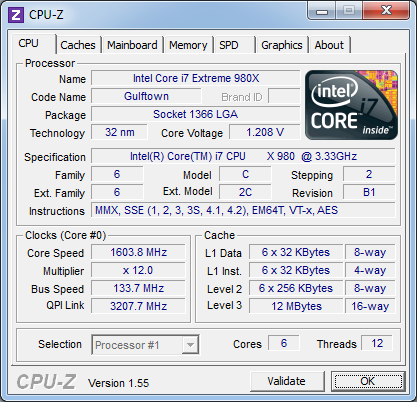
\includegraphics[scale=1]{imgs/cpu-z.png} 
\end{center}

%%%%%%%%%%%%%%%%%%%%%%%%%%%%%%%%%%%%%%%%%%%%%%%%%%%%%%%%%%%%%%%%

\newpage
\section{Трассировка лучей}
Классический ray tracing~[\cite{sivakov}], или метод трассировки лучей, предложен Артуром Аппелем (Arthur Appel) еще аж в 1968 году и дополнен алгоритмом общей рекурсии, разработанным Whitted в 1980 году. Понадобилось почти 12 лет эволюции вычислительных систем, прежде чем этот алгоритм стал доступен для широкого применения в практических приложениях. Реализация высокопроизводительной версии трассировки лучей уже предпринимаются различными компаниями. О сложности задачи трассировки лучей можно прочитать в соответствующих источниках~[\cite{biovulf}].

\subsection{Алгоритмы трассировки лучей}
Суть метода заключается в отслеживании траекторий лучей и расчета взаимодействий с лежащими на траекториях объектами, от момента испускания лучей источником света до момента попадания в камеру. Под взаимодействием луча с объектами понимаются процессы диффузного (в смысле модели локальной освещенности), многократного зеркального отражения от их поверхности и прохождение лучей сквозь прозрачные объекты. Таким образом, ray tracing – первый метод расчета глобального освещения, рассматривающий освещение, затенение (расчет тени), многократные отражения и преломления. Различают два основных вида метода трассировки лучей: \textbf{\textit{прямой}} -- \index{forward ray tracing}forward ray tracing, и \textbf{\textit{обратный}} -- \index{backward ray tracing}backward ray tracing.

\subsubsection{Прямой метод трассировки лучей}
В прямом методе траектории лучей строятся от источника ко всем точкам всех объектов сцены (первичные лучи). Затем проверяется ориентация каждой точки относительно источника, и, если она лежит на стороне объекта, обращенной в противоположную от источника сторону, точка из расчетов освещенности исключается. Для всех остальных точек вычисляется освещенность с помощью локальной модели освещения. Если объект не является отражающим или прозрачным, то есть поверхность объекта только диффузно рассеивает свет, траектория луча на этой точке обрывается (заканчивается). Если же поверхность объекта обладает свойством отражения (\index{reflection}reflection) и/или преломления (\index{refraction}refraction), из точки строятся новые лучи, направления которых совершенно точно определяются законами отражения и преломления.
\par
    Для построенных таким образом траекторий новых лучей может быть только три исхода. Луч либо выходит за пределы видимой из камеры области сцены, в этом случае все проделанные для него до этого момента расчеты освещенности отбрасываются, поскольку они не принимают участия в формировании изображения. Или луч попадает в камеру, тогда рассчитанная освещенность формирует цвет соответствующего пиксела изображения. Или луч встречает на своем пути новый
объект, тогда для новой точки пересечения повторяется расчет освещенности и построения лучей отражения и преломления в зависимости от свойств поверхности объекта (рекурсия). Построение новых траекторий и расчеты ведутся до тех пор, пока все лучи либо попадут в камеру, либо выйдут за пределы видимой области. Очевидно, что при прямой трассировке лучей мы вынуждены выполнять расчеты для лучей, которые не попадут в камеру, то есть, проделывать бесполезную работу. По некоторым оценочным данным доля таких "слепых"лучей довольно велика. Эта главная, хотя и далеко не единственная, причина того, что метод прямой трассировки лучей считается неэффективным и на практике не используется(в чистом виде).

\subsubsection{Обратный метод трассировки лучей}
Обратной метод трассировки лучей, или backward ray tracing. Этот метод расчетов основывается на построении лучей от наблюдателя через плоскость экрана вглубь сцены, а не от источника, то есть -- наоборот. Этот способ достаточно изящен, что позволяет решить массу проблем, возникающих при прямой трассировке, а сам метод отличается простотой и понятностью. Лучи теперь строятся иначе. А именно, по двум точкам: первая точка, общая для всех лучей – положение камеры (наблюдателя), вторая точка определяется положением пиксела на плоскости видового окна. Таким образом, направление каждого луча строго определено (две точки в пространстве определяют одну и только одну прямую – школьный курс геометрии), и количество первичных лучей также известно – это общее количество пикселей видового окна. Например, если видовое окно имеет 1920 пикселей по ширине и 1200 пикселей по высоте, количество лучей составит 1920 х 1200 = 2 304 000. Каждый луч
вдоль заданного направления продлевается от наблюдателя вглубь трехмерной сцены, и для каждой траектории выполняется проверка на пересечение со всеми объектами сцены и с отсекающими плоскостями. Если пересечений с объектами нет, а есть пересечение только с плоскостью отсечения, значит луч выходит за пределы видимой части сцены, и соответствующему пикселю видового окна присваивается цвет фона. Если луч пересекается с объектами сцены, то среди всех объектов выбирается тот, который ближе всего к наблюдателю. В точке пересечения с таким объектом строится три новых, так называемых вторичных луча. \par

\begin{center}
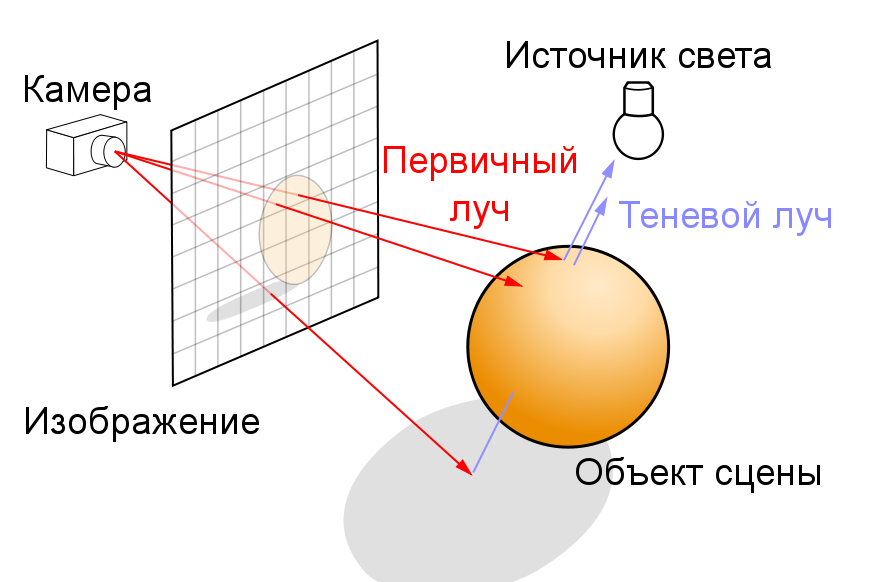
\includegraphics[scale=0.5]{imgs/Ray_trace_diagram_rus.png} 
\end{center}

Первый луч строится в направлении источника света. Если источников несколько, строится несколько таких лучей, по одному на каждый источник. Основное назначение этого луча – определить ориентацию точки (обращена точка к источнику или от него), наличие объектов, закрывающих точку от источника света, и расстояние до источника света. Если точка обращена в противоположную сторону от источника света или закрыта другим непрозрачным объектом, освещенность от такого источника не рассчитывается, точка находится в тени. В случае затеняющего прозрачного объекта интенсивность освещения уменьшается в соответствии со степенью прозрачности. Если точка закрыта от освещения всеми источниками сцены, ей присваивается фоновый (\index{ambient или фоновый цвет}ambient) цвет. В противном случае точка освещена, интенсивность и цвет освещения рассчитываются при помощи локальной модели освещенности, как сумма освещенностей от всех источников, для которых эта точка не закрыта другими объектами. Этот тип луча получил название \index{shadow ray или теневой луч} \textit{\textbf{shadow ray}} (иногда его еще называют \index{illumination ray}illumination ray) – теневой луч. Если поверхность объекта не является отражающей и непрозрачна, теневой луч – единственный тип лучей который строится, траектория первичного луча обрывается (заканчивается), и дальнейшие расчеты не выполняются. Рассчитанный цвет (освещенности или тени) присваивается тому пикселю видового окна, через который проходит соответствующий первичный луч.
   \par
   Второй луч строится, если поверхность объекта обладает отражающими свойствами, и называется \index{reflection ray или отраженный луч} reflection ray, или луч отражения. Направление отраженного луча определяется по закону:
$$
	\vec{R} = \vec{I} - 2 \cdot \vec{N} (\vec{N} , \vec{I})
$$
где $\vec{R}$ - отраженный луч, $\vec{I}$ - падающий пераичный луч, $\vec{N}$ - нормаль к поверхности в точке соударения.
Для отраженного луча проверяется возможность пересечения с другими объектами сцены. Если пересечений нет, то интенсивность и цвет отраженного луча равна интенсивности и цвету фона. Если пересечение есть, то в новой точке снова строится три типа лучей – теневые, отражения и преломления.
Третий луч строится, если поверхность объекта прозрачна, и носит название \index{transparency ray или преломленный луч}transparency ray, т. е. луч преломленный. Направление для преломленного луча определяется следующим образом:
$$
 \vec{T} = \frac{n_1}{n_2} \cdot \vec{I} - \left[ \cos \alpha + \frac{n_1}{n_2} \cdot \left(\vec{N},\vec{I} \ \right) \right] \cdot \vec{N}
$$
$$
\cos \alpha = \sqrt{1 - \left( \frac{n_1}{n_2} \right) ^2 \cdot \left(1-\left(\vec{N},\vec{I}\ \right)^2\right)}
$$
где $\vec{T}$ - переломленный луч, $n_1$ - коэффициент рефракции для первой среды ( в которой растространяется первичный луч ), $n_2$ - коэффициент рефракции для второй среды прозрачного объекта.

Так же, как и в предыдущем случае, проверяется пересечение вновь построенного луча с объектами, и, если они есть, в новой точке строятся три луча, если нет -- используется интенсивность и цвет фона.

Таким образом, для каждого первичного луча можно построить древовидную структуру. Если древовидная структура для данного луча построена, то расчет освещенности можно выполнить в следующем порядке. Для каждой ветви дерева спускаемся вдоль древовидной структуры к последнему пересечению вторичного луча и поверхности (будем дальше называть их узлами). Поскольку это последний узел в цепи, то  вкладов от преломлений и отражений нет, поэтому, освещенность узла вычисляется при помощи локальной модели освещения с учетом видимости источников света для данного узла. Затем, вычисленная освещенность передается вверх по ветви к следующему ближайшему узлу. Освещенность в этом узле будет вычисляться по формуле:

$$
 \vec{I}_{total} = \vec{I}_{local} + K_{reflection} \cdot \vec{I}_{reflection} + K_{refraction} \cdot \vec{I}_{refraction}
$$

где $\vec{I}_{total}$ - полная освещенность в точке, $\vec{I}_{local}$ - локальная освещенность в точке, вычисленная от источников освещения с помощью одной из локальной модели освещенности, $K_{reflection}$ - коэффициент, определяющий отражающие свойства поверхности, $\vec{I}_{reflection}$ - освещенность предыдущей точки, переданная вдоль ветки отражения,   $K_{refraction}$ - коэффициент, определяющий преломляющие свойства поверхности $\vec{I}_{refraction}$ - освещенность предыдущей точки, переданная вдоль ветки преломления

Естественным завершением трассировки лучей является выход всех испущенных вторичных лучей за пределы видимой области и их рассеяние на чисто диффузных объектах. Результат вычислений будет наиболее точным. Но, если сцена достаточно сложна, такой расчет будет очень медленным, а в некоторых случаях и невозможным по причине ограниченности аппаратных ресурсов. Легко увидеть, что вклад освещенности от каждого нового вторичного луча очень быстро уменьшается по той простой причине, что коэффициенты свойств отражения и преломления материалов меньше единицы. Поэтому часто трассировку лучей прекращают, когда вклад от следующего узла ветви становится меньше заданной величины. Это также достаточно точный метод расчетов, который может быть использован для получения качественных результатов при определенных условиях. Наконец, для получения оценочного расчета можно оборвать трассировку лучей после выполнения заданного количества итераций, это самый быстрый и наименее точный расчет.

\subsubsection{Достоинства и недостатки}

Основные достоинства рекурсивного метода обратной трассировки лучей – расчет теней, многократных отражений и преломлений, значительно повысивших степень реалистичности получаемых изображений.
Основные недостатки: неучет вторичного освещения от диффузно отраженного объектами света; низкая скорость и высокая вычислительная стоимость расчетов – в классическом рейтресинге необходимо проверять на пересечение каждый луч со всеми объектами сцены, в результате от 70 до 95 процентов всего времени расчетов тратится на вычисление пересечений; резкие границы цветовых переходов тени/подсветок/прозрачности; \index{aliasing}aliasing – "зазубренность" линий и т. д.; дискретность определяющих цвет пиксела первичных лучей – одного первичного луча недостаточно для корректного определения цвета пиксела, формирующего изображение.


\subsection{Модели освещения}

В соответствии с принятым в компьютерной графике подходом, расчет освещенности распадается на две основные задачи. Первая – определить способ расчета освещенности в произвольной точке трехмерного пространства, решается при помощи построения обобщенной математической модели освещенности (Illuminating model). Вторая задача – применение Illuminating model для компьютерных расчетов освещенности трехмерных объектов с конкретной геометрией и свойствами поверхности, решается при помощи так называемой модели затенения (Shading model).

Моделей освещенности к настоящему моменту разработано несколько. Самая первая,и самая простая – локальная модель освещенности. Эта модель не рассматривает процессы светового взаимодействия объектов сцены между собой, а только расчет освещенности самих объектов. Вторая, глобальная модель освещенности – Global Illuminations, рассматривает трехмерную сцену как единую систему и пытается описывать освещение с учетом взаимного влияния объектов. В рамках этой модели рассматриваются такие вопросы, как многократное отражение и преломление света (ray tracing), рассеянное освещение (radiosity), каустик(caustic) и фотонные карты (photon mapping) и другие. 

\subsubsection{Глобальные модели освещения}

Глобальное освещение (global illumination) — это название ряда алгоритмов, используемых в 3D-графике, которые предназначены для добавления более реалистичного освещения в трёхмерные сцены. Такие алгоритмы учитывают не только свет, который поступает непосредственно от источника света (прямое освещение, англ. direct illumination), но и такие случаи, в которых лучи света от одного и того же источника, отражаются на других поверхностях сцены (непрямая освещенность, англ. indirect illumination).

Теоретически отражение, преломление, тень — примеры глобального освещения, потому что, для их имитации необходимо учитывать влияние одного объекта на другие (в отличие от случая когда на объект падает прямой свет). На практике, однако, только моделирование диффузного отражения или каустики называется глобальным освещением.

Изображения полученные в результате применения алгоритмов глобального освещения часто кажутся более фотореалистичными, чем те, в процессе рендеринга которых применялись алгоритмы только прямого освещения, но для просчета глобального освещения требуется гораздо больше времени.

\subsubsection{Локальные модели освещения}

Существующие локальные модели освещения можно разделить на две категории. К первой категории относятся эмпирические модели. Они обычно эффективны в плане быстродействия и некоторые из них дают довольно реалистичную картинку. Они обычно не оперируют такими физическими величинами, как световая энергия, или световой поток. Однако эти модели находят довольно широкое применение в областях, где не требуется точная физическая информация об освещении (например, спецэффекты в фильмах, программы для художников и дизайнеров, для рекламных целей)

Ко второй категории относятся модели, базирующиеся на физических представлениях о теории света. Изображения, полученные с использованием этих моделей, очень хорошо соотносятся с экспериментальными данными. Поэтому эти модели находят применение там, где важна точная имитация поведения света (оформление интерьеров, архитектура)

\subsubsection{Модель Фонга}

Это эмпирическая модель. В самом общем случае, в свете требования фотореалистичности, эта модель учитывает и неявное ambient-освещение. Ambient-освещение, или его еще называют фоновым (background), – это окружающее объект освещение от удаленных источников, чье положение и характеристики не известны. Необходимость учета ambient-освещения, пусть и очень грубо, обусловлена тем, что его вклад может быть достаточно велик – до 50\% от общей освещенности. В Local Illumination считают, что фоновое освещение задает цвет (и его интенсивность) объекта в отсутствии явных источников света или в тени. Не несет никакой информации об объекте, кроме значения простого цвета, равномерно заливающего контур объекта.

Интенсивность такого освещения постоянна и равномерно распределена во всем пространстве, расчет его отражения поверхностью выполняется по формуле:

$$
 \vec{I}_{amb} = K_{a} \cdot \vec{I}_{a}
$$

где $\vec{I}_{amb}$  - интенсивность отраженного ambient освещения, $K_{a}$ - коэффициент, характеризующий отражающие свойства поверхности для  ambient-освещения, $\vec{I}_{a}$ - исходная интенсивность ambient-света, падающего на поверхность.

Часть света от прямых источников зеркально отражается поверхностью, а остальной свет диффузно рассеивается во всех направлениях. Кроме чисто зеркального отражения, которое имеют идеально отполированные поверхности, различают так называемое glossiness или распределенное зеркальное отражение – отражение в некотором створе углов, а не на один единственный угол. Такое рассеяние света обусловлено микрорельефом ("шероховатостью") поверхности, то есть поверхность реальных объектов не является идеально гладкой, а состоит из большого количества микровыступов и впадин, которые зеркально отражают падающий свет под разными углами. Результатом glossy-отражения является specular highlight – яркий световой блик, имеющий размер в зависимости от степени шероховатости поверхности. 

Интенсивность рассеянного света зависит от угла падающего на поверхность света по закону Ламберта (Lambert):

$$
 \vec{I}_{diff} = K_{diff} \cdot \vec{I}_{d} \cdot \cos(\alpha)
$$
 
где $\vec{I}_{d}$ - интенсивность падающего на поверхность света, $K_{diff}$ - коэффициент, характеризующий рассеивающие свойства поверхности, $\cos(\alpha)$ - угол между направлением на источник света и нормалью поверхности

Другими словами, поверхность будет освещена больше, если свет падает на нее перпендикулярно ($\alpha = 0$), и меньше, если свет падает под любым другим углом, поскольку в этом случае увеличивается освещаемая площадь. Диффузно рассеянный свет является главным источником визуальной информации о геометрии трехмерных объектов.

Как было уже сказано ранее, свет отражается зеркально в некотором створе углов, и для большинства реальных материалов мы всегда видим зеркальную подсветку в форме светового пятна, а не в форме яркой точки. Поэтому, для расчета интенсивности зеркально отраженного света используется формула, предложенная Фонгом:

$$
 \vec{I}_{spec} = K_{spec} \cdot \vec{I}_{s} \cdot \cos^n(\beta)
$$

где $\vec{I}_{spec}$ - интенсивность зеркально отраженного света,  $\vec{I}_{s}$ - интенсивность источника света,  $\vec{K}_{s}$ - коэффициент, характеризующий свойства зеркального отражения поверхности
$\beta$ - угол между направлением идеального отражения и направлением на наблюдателя, степень $n$ определяет размер пятна светового блика, чем больше $n$, тем меньше световой блик, и тем ближе отражающие свойства поверхности к свойствам идеального зеркала.

Формула Фонга – пример компьютерной фикции, поскольку она не имеет физического смысла. Ее используют просто потому, что она дает хорошие практические результаты. 

Таким образом, локальная модель освещенности предполагает расчет отраженной фоновой освещенности, диффузного и зеркального отражения от прямых источников: 

$$
 \vec{I}_{local} =  K_{amb} \cdot \vec{I}_{amb} +  K_{diff} \cdot \vec{I}_{diff} \cdot \left( \vec{L},\vec{N} \right) + K_{spec} \cdot \vec{I}_{spec} \cdot \left( \vec{R},\vec{V} \right)^n
$$



\subsection{Примитивы}
\subsubsection{\index{Плоскость}Плоскость}
Для определения пресечения луча с плоскостью, необходимо найти точку в пространстве, которая будет удовлетворять двум уравнениям: уравнению луча и уравнению плоскости.
\par
Уравнение луча:
\begin{equation}
\left\{
\begin{array}{ccccc}
x & = & x_0 & + & t \cdot x_d \\
y & = & y_0 & + & t \cdot y_d \\
z & = & z_0 & + & t \cdot z_d \\
\end{array}
\right.
\label{equation_ray}
\end{equation}
или
$$
\vec{R}(t) = \vec{O} + t \cdot \vec{D}
$$
где $O = \VECXYZ{0} $ - начало луча, а $D = \VECXYZ{d} $ - направление луча. 
\par
Уравнение плоскости задается следующим образом:
\begin{equation}
Ax + By + Cz + D = 0
\label{equation_plane}
\end{equation}
\par
Для того, что бы найти точку пересечения луча с плоскостью, необходимо подставить уравнение (\ref{equation_ray}) в (\ref{equation_plane}):
$$
A(x_0 + t \cdot x_d) + B(y_0 + t \cdot y_d) + C(z_0 + t \cdot z_d) + D = 0
$$
Раскроем скобки и приведем подобные
$$
t(Ax_d + By_d + Cz_d ) + Ax_0 + By_0 + Cz_0 + D = 0
$$
найдем неизвестную величину t
$$
 t = - \frac{Ax_0 + By_0 + Cz_0 + D}{Ax_d + By_d + Cz_d}
$$
из уравнения видно, что луч либо пересекает плоскость в какой то точке, либо нет. Это связано с тем, что если $Ax_d + By_d + Cz_d = 0$, то плоскость и луч параллельны друг другу. Т.к. $P = \VEC{A}{B}{C} $ - это нормаль к поверхности, то из геометрии известно, что если $( D , P ) = 0$, то вектора параллельны.
\par
   Для того, что бы найти величину $t$, необходимо рассчитать всего несколько скалярных произведений:
$$
t = - \frac{(O, P) + D}{(D, P)}
$$
при условии, что $(D, P) \neq 0$

\subsubsection{\index{Сфера}Сфера}
Для сферы необходимо проделать те же выкладки.
Уравнение луча:
\begin{equation}
\left\{
\begin{array}{ccccc}
x & = & x_0 & + & t \cdot x_d \\
y & = & y_0 & + & t \cdot y_d \\
z & = & z_0 & + & t \cdot z_d \\
\end{array}
\right.
\label{equation_ray}
\end{equation}
или
$$
\vec{R}(t) = \vec{O} + t \cdot \vec{D}
$$
Уравнение сферы записывается следующем образом:
\begin{equation}
(x-x_c)^2 + (y-y_c)^2 + (z-z_c)^2 = r^2
\label{equation_sphere}
\end{equation}
где $S = \VECXYZ{c}$ - центр сферы, а $r$ - радиус. Подставим уравнение (\ref{equation_ray}) в (\ref{equation_sphere}):
$$
\left( (x_0 + t \cdot x_d) - x_c \right)^2 + 
\left( (y_0 + t \cdot y_d) - y_c \right)^2 + 
\left( (z_0 + t \cdot z_d) - z_c \right)^2 = r^2
$$
приведем это уравнение в виду
\begin{equation}
A \cdot t^2 + B \cdot t + C = 0
\label{equation_square}
\end{equation}
после раскрытия скобок и приведения подобных, получаем:
\par
$$
A = x^2_d + y^2_d + z^2_d
$$ 
\par
$$
B = 2x_d(x_0 - x_c) + 2y_d(y_0 - y_c)  + 2z_d(z_0 - z_c) 
$$ 
\par
$$
C = (x_0 - x_c)^2 + (y_0 - y_c)^2 + (z_0 - z_c)^2 
$$
Если уравнение (\ref{equation_square}) не имеет вещественных решений, то луч не пересекает сферу. Если имеется два решения, то наименьший положительный корень этого уравнения определит на луче ближайшую точку пересечения луча со сферой.
\par
Рассмотрим подробнее как вычисляются коэффициенты $A$, $B$, $C$:
\par
$$
A = x^2_d + y^2_d + z^2_d = (D, D)
$$ 
\par
$$
B = 2x_d(x_0 - x_c) + 2y_d(y_0 - y_c)  + 2z_d(z_0 - z_c)  = 2 \cdot (D, D - S)
$$ 
\par
$$
C = (x_0 - x_c)^2 + (y_0 - y_c)^2 + (z_0 - z_c)^2 = (O - S, O - S )
$$
Далее решаем обыкновенное квадратное уравнение и находим корни и получаем значение $t$
$$
t_{1,2} = \frac{-B \pm \sqrt{B^2 - 4 \cdot A \cdot C}}{2 \cdot A}
$$

$$
t_{1} = \frac{ - 2 \cdot (\vec{D}, \vec{D} - \vec{S}) + \sqrt{(2 \cdot (\vec{D}, \vec{D} - \vec{S}))^2 - 4 \cdot (\vec{D}, \vec{D}) \cdot (\vec{O} - \vec{S}, \vec{O} - \vec{S} )}}{2 \cdot (\vec{D}, \vec{D})}
$$

$$
t_{2} = \frac{ - 2 \cdot (\vec{D}, \vec{D} - \vec{S}) - \sqrt{(2 \cdot (\vec{D}, \vec{D} - \vec{S}))^2 - 4 \cdot (\vec{D}, \vec{D}) \cdot (\vec{O} - \vec{S}, \vec{O} - \vec{S} )}}{2 \cdot (\vec{D}, \vec{D})}
$$

\subsubsection{\index{Треугольник}Треугольник}
Алгоритм пересечения луча и треугольника основан на барицентрических координатах.
\par
Барицентрические координаты -- координаты точки $n$-мерного аффинного пространства $A^n$, отнесенные к некоторой фиксированной системе из $(n + 1)$-ой точки $p_0, p_1, \dots, p_n$ , не лежащих в $(n -1)$-мерном подпространстве. Пусть $z$ есть произвольная точка в $A^n$. Каждая точка $x \in A^n$ может быть единственным образом представлена в виде суммы
$$
	x = z + \alpha_1 \cdot z\vec{p_1} + \alpha_2 \cdot z\vec{p_2} + \cdots + \alpha_n \cdot z\vec{p_n} 
$$
где $\alpha_1, \alpha_2, \dots,  \alpha_n $ вещественные числа, удовлетворяющие условию
$$
\alpha_1 + \alpha_2 + \cdots + \alpha_n  = 1
$$
Числа $\alpha_1, \alpha_2, \dots,  \alpha_n $ называются барицентрическими координатами точки $x$. Легко видеть, что барицентрические координаты не зависят от выбора $z$.

Точка $T(u,v)$, принадлежащая треугольнику, может быть записана в виде:
\begin{equation}
\label{triangle_bar}
T(u,v) = (1-u-v)V_0 + uV_1 + vV_2
\end{equation}

\noindent где $(u,v)$ -- это бариецентрические координаты такие, что $u \geq 0$, $v \geq 0$ и $u + v \leq 1$

Вычисление пересечения между лучем(\ref{equation_ray}) и треугольником(\ref{triangle_bar}), это решение следующего уравнения:

$$
O + tD = (1-u-v)V_0 + uV_1 + vV_2
$$

\noindent после нескольких очевидных преобразований:

$$
O + tD = V_0 - uV_0 - vV_0 + uV_1 + vV_2
$$
$$
O - V_0 = - tD + uV_1 - uV_0 + vV_2 - vV_0
$$

$$
- tD + u(V_1 - V_0) + v(V_2 - V_0) = O - V_0
$$

\noindent получаем:

\begin{equation}
\label{ray_cross_tr}
\left[ -D, V_1 - V_0 , V_2 - V_0\right] 
\left[  
\begin{array}{c} t \\ u \\ v \\ \end{array}
\right] = O - V_0
\end{equation}

Что бы решить задачу, необходимо найти вектор $\VEC{t}{u}{v}$. Обозначив $E_1 = V_1 - V_0$, $E_2 = V_2 - V_0$ и $T = O - V_0$ решим уравнение (\ref{ray_cross_tr}), используя метод Крамера:

\begin{equation}
\label{ray_cross_tr_solv}
\left[  
\begin{array}{c} t \\ u \\ v \\ \end{array}
\right] = 
\frac{1}{| -D , E_1, E_2|} 
\left[  
	\begin{array}{lcccl}
	|& T , & E_1, &E_2 & | \\
	|&-D , & T  , &E_2 & | \\
	|&-D , & E_1, &T   & | \\
	\end{array}
\right] 
\end{equation}

\noindent Из курса линейной алгебры известно, что: $|A, B, C| = - (A \times C) \cdot B = - (C \times B) \cdot A$. Принимая во внимания этот факт, перепишем уравление (\ref{ray_cross_tr_solv}).

\begin{equation}
\label{ray_cross_tr_solv2}
\left[  
\begin{array}{c} t \\ u \\ v \\ \end{array}
\right] = 
\frac{1}{(D \times E_2)\cdot E_1} 
\left[  
	\begin{array}{c}
	(T \times E_1) \cdot E_2 \\
	(D \times E_2) \cdot T \\
	(T \times E_1) \cdot D \\
	\end{array}
\right] = 
\frac{1}{P \cdot E_1} 
\left[  
	\begin{array}{c}
	Q \cdot E_2 \\
	P \cdot T \\	
	Q \cdot D \\	
	\end{array}
\right]
\end{equation}
где $P = (D \times E_2)$ и $Q = T \times E_1$


%%%%%%%%%%%%%%%%%%%%%%%%%%%%%%%%%%%%%%%%%%%%%%%%%%%%%%%%%%%%%%%%%%%%%%%%%%%%%%%%%%%%%%%%%%%

\newpage
\section{Оптимизация}
Оптимизация -- как способ программирования по уровням архитектуры сверху вниз.

\subsection{Шаблоны C++}

\subsubsection{Понятие шаблона}

Шаблоны(Templates) были введены в язык C++ как средство, позволяющие параметризовать типы данных. Это связано с тем, что для классов или функций приходилось реализовывать одни и те же алгоритмы, но для разных типов данных. Получали дублирование кода, и тем самым росло число ошибок. 
Пример. Реализовать функцию, которая возвращает максимальное значение из 2 чисел.

\cppsource{src/deftemplate.tex}{Несколько реализация функции {\bf max}}

\noindent
и так далее. Приходится писать один и тот же код несколько раз. Во второй функции можно было допустить ошибку (например указать неправильный знак сравнения), которую потом очень трудно найти. Или наоборот, после обнаружения ошибки, придется править код во всех реализациях функции max (возможна ситуация, когда в нескольких местах ошибка была исправлена, а в остальных пропущена или забыта). С этими проблемами помогли справится шаблоны, которые параметризовали типы данных следующим образом:

\cppsource{src/definetemplate.tex}{Шаблонное определение функции {\bf max}}

%\noindent
Т. о. работу которую выполнял программист теперь выполняет компилятор. При вызове функции, в качестве параметров которых нужно сравнить два int, компилятор сам из шаблона выведет функцию max(int,int).
\subsubsection{Вычисление на шаблонах}
Сегодня шаблоны используют различным образом, не так как ожидали изобретатели
шаблонов С++. Сегодня программирование на шаблонах включают различные техники, такие как: обобщенное программирование, вычисление во время компиляции, шаблонные выражения(expression templates), мета-программирование, и др.

\noindent Рассмотрим пример вычисления факториала. \\
\noindent Факториал числа N это: $N! = N \cdot (N-1) \cdot \dots \cdot 1$

Рекурсивная реализация факториала, без использование шаблонов, приведена в следующем листинге:

\cppsource{src/rekfactorial.tex}{Рекурсивная реализация факториала}

Эту функцию следует использовать следующим образом:
\begin{verbatim}
cout << factorial(7) << endl;
\end{verbatim}
Вызывать рекурсивно функцию - это очень большие накладные расходы. Несмотря на то, что мы указало компилятору встроить функцию (inline), компилятор проигнорирует это, так как он не может сделать постановку в рекурсию. Можно добиться большего успеха, если реализовывать это, как класс с шаблоном.

\cppsource{src/templatefactorial.tex}{Реализация факториала на шаблонах}

Можно заметить, что у данного шаблона нет ни данных, ни функциональных участков, это только определение перечислимого типа. Для того чтобы можно было определить шаблон для n, нужно для начала определить шаблон для n-1, т. е. для n-2, n-3 и т. д. В итоге получаем рекурсию. Следует заметить, что в качестве параметра шаблона используется обычный тип int. По стандарту, в качестве параметров шаблона могут быть использованы только перечислимые типы. В нашем случае есть параметр шаблона типа int, это означает, что в этот шаблон будет подставлено постоянное число типа int. Что бы воспользоваться данным классом необходимо написать следующие:
\begin{verbatim}
cout << factorial<7>::ret << endl;
\end{verbatim}
Компилятор рекурсивно определяет значение факториала<7>, затем <6> и так далее. Так как это рекурсия, то что бы не зациклится необходимо вовремя остановится. Любая рекурсия нуждается в остановки, и это не исключение. Это можно сделать с помощью специализации шаблона(т.е. определение для частного случая).

\cppsource{src/specfactorial.tex}{Специализация шаблона вычисления факториала}

Когда компилятор начнет определять специализацию для <0>, то он подставит имеено эту реализацию и рекурсия завершится. В результате, получится следующая структура:

\cppsource{src/finfactorial.tex}{Развернутая структура вычисления факториала}

Как видно из примера, от структуры уже ничего ни осталось и при уровне оптимизации начиная с O1, компилятор подсчитает выражение и вместо:
\begin{verbatim}
cout << factorial<7>::ret << endl;
\end{verbatim}
Подставит, подсчитанное выражение:
\begin{verbatim}
cout << 5040 << endl;
\end{verbatim}
Проверить это можно дизассемблировав данный пример и увидеть в коде число 5040.

\subsection{SIMD инструкции}
Применение SIMD инструкций в классе vec4.

\subsection{Ускоряющие структуры}
BVH. Алгоритмы построения и поиска.

%%%%%%%%%%%%%%%%%%%%%%%%%%%%%%%%%%%%%%%%%%%%%%%%%%%%%%%%%%%%%%%%%%%%%%%%%%%%%%%%%%%%%%%%%%%

\newpage
\section{Постановка и результаты экспериментов}

Эксперименты проводилимь на 6 ядерном компьютере с процессором Intel Core i7 980x с частотой 3.33GHz, оперативной памятью 12 Гб, ОС - Calculate Linux 11.0 x64. 

Для сборки приложения с библиотекой tbb, необходимо, что бы компилятор поддерживал лямбда выражения из нового стандарта c++0x. На данный момент, этот стандарт поддерживает компилятор GCC 4.5.2

\subsection{Timer}
Для того, чтобы точно оценивать время работы каждого из алгоритмов, очень важно иметь такой инструмент как таймер, способный оценить время работы алгоритма. 
Проблема в том, что стандарные методы операционных систем не работают с нужной точностью. Когда идет речь о том, чтобы оценить время, который должен исполнятся очень много миллионов раз в секунду, важен каждый такт процессора и точность в миллисекунду и уж тем более в секундах просто неприемлема.

Для очень точной оценки времени работы алгоритмов, был специально написан высокоточный таймер на языке c++, с использованием ассемблера (AT\&T - синтаксиса).
Таймер выдает время в тактах процессора и включает в себя разные режимы подсчета времени.

\subsubsection{Алгоритм работы высокоточного таймера}

\cppsource{src/timer.tex}{Метод Start() и Stop() класса Timer}


\subsubsection{Эксперименты с высокоточным таймером}

\subsection{Вектора и Expression templates}

\subsection{Тестовая сцена}

\subsection{Эффективность расспаралеливания}

\subsection{TBB vs OpenMP}

\subsection{Влияние SIMD инструкций на скорость работы}

\subsection{Компилирование высокоуровнего кода в ассемблер}

Ассемблерные вставки, которые показывают что вычисление отражающего луча это одно SSE.

%%%%%%%%%%%%%%%%%%%%%%%%%%%%%%%%%%%%%%%%%%%%%%%%%%%%%%%%%%%%%%%%%%%%%%%%%%%%%%%%%%%%%%%%%%%

\newpage
\section*{Заключение}
\addcontentsline{toc}{section}{Заключение} 
Задача трассировки лучей является по настоящему трудным испытанием для центрального процессора. Несмотря на то, что процессор обладает хорошей производительностью на ядро, общей производительности ему не хватает. Несмотря на столь малые мощности, удалось реализовать достаточно быстрый алгоритм на центральном процессоре. Для большей производительности была разработана эффективная параллельная версия программы с использованием библиотеки TBB и
стандарта параллельного OpenMP. Благодаря использованию языка с++ и технику шаблонных выражений, удалось еще повысить производительность программы. Программа продемонстрировала хорошую производительность: используя всего лишь один процессор можно получать изображения в реальном времени.

%%%%%%%%%%%%%%%%%%%%%%%%%%%%%%%%%%%%%%%%%%%%%%%%%%%%%%%%%%%%%%%%%%%%%%%%%%%%%%%%%%%%%%%%%%%

\newpage
\begin{thebibliography}{99}
	\bibitem{morozov_kazan} Морозов А. С. Трассировка лучей в реальном времени на многоядерном процессоре. Высокопроизводительные параллельные вычисления на кластерных системах (HPC-2008). Материалы Восьмой Международной конференции-семинара. Казань, ноябрь 17-19, 2008. Труды конференции — Казань: Изд. КГТУ, 2008. - С. 241.
	\bibitem{morozov_microsoft} Морозов А. С. Высокопроизводительная реализация трассировки лучей с использованием Microsoft MPI. Технологии Microsoft в теории и практике программирования. Материалы конференции /Под ред. Проф. В.П. Гергеля. - Нижний Новгород: Изд-во Нижегородского госуниверситета, 2009. - 527 с.
	\bibitem{morozov_pavt} Морозов А. С. Сравнительный анализ алгоритма трассировки лучей на системах с общей и разделяемой памятью. Параллельные вычислительные технологии (ПаВТ’2009): Труды международной научной конференции (Нижний Новгород, 30 марта - 3 апреля 2009 г.). - Челябинск: Изд. ЮурГУ, 2009. - 839 с
	\bibitem{latex} Львовский С.М. Набор и верстка в системе \LaTeX. – 4-е изд., стереотипн. – М.: МЦНМО, 2006
	\bibitem{alloftex} Кнут, Дональд, Э. Все про \TeX. : Пер. с англ. --- М. : Издательский дом ''Вильямс'', 2003. --- 560 с. : ил. --- Парал. Тит. англ.
	\bibitem{inteloptimize} Гербер Р., Бик А., Смит К., Тиан К. Оптимизация ПО. Сборник рецептов. --- СПб.: Питер, 2010. --- 352 с.: ил. --- (Серия ''Библиотека программиста'').
	\bibitem{templatecpp} Вандевурд, Дэвид, Джосаттис, Николаи М. Шаблоны C++: справочник разработчика. : Пер. с англ. --- М. : Издательский дом ''Вильямс'', 2008. --- 544 с. : ил. --- парал. тит. англ.
	\bibitem{straustrupcpp} Б. Страуструп Язык программирования C++. Специальное издание / Пер. с англ. --- М.: ООО ''Бином-Пресс'', 2006. --- 1104 с.: ил.
	\bibitem{sivakov} Сиваков И. Как компьютер рассчитывает изображения. Технология программного рендеринга, 11.03.2004. \\ (\href{http://www.fcenter.ru/online.shtml?articles/hardware/videos/8749}{http://www.fcenter.ru/online.shtml?articles/hardware/videos/8749})
	\bibitem{biovulf} Дмитрий Мороз. "Беовульф": Создание фильма, 11.12.2007.\\ (\href{http://www.3dnews.ru/editorial/beowulf}{http://www.3dnews.ru/editorial/beowulf})
	\bibitem{intelintrinsic} Intel® C++ Intrinsics Reference \\ (\href{http://www.intel.com/products/processor/manuals/}{http://www.intel.com/products/processor/manuals/})
	\bibitem{intelmanual} Intel 64 and IA-32.Architectures Software Developer's Manual \\ (\href{http://www.intel.com/products/processor/manuals/}{http://www.intel.com/products/processor/manuals/})
	\bibitem{tbbtutor} Intel® Threading Building Blocks. Tutorial \\ (\href{http://www.threadingbuildingblocks.org/}{http://www.threadingbuildingblocks.org/})
	\bibitem{tbbmanual} Intel® Threading Building Blocks. Reference Manual \\ (\href{http://www.threadingbuildingblocks.org/}{http://www.threadingbuildingblocks.org/})
	\bibitem{cppexpressiontemplate} C++ Expression Templates An Introduction to the Principles of Expression Templates, 2003 \\ (\href{http://www.angelikalanger.com/Articles/Cuj/ExpressionTemplates/ExpressionTemplates.htm}{http://www.angelikalanger.com/.../ExpressionTemplates.htm})
	\bibitem{intelcore980x} Шесть ядер для десктопа: Intel Core i7-980X Extreme Edition, 07.04.2010 \\ (\href{http://www.fcenter.ru/online.shtml?articles/hardware/processors/28480}{http://www.fcenter.ru/online.shtml?articles/hardware/processors/28480})
	\bibitem{rdtscp} How to Benchmark Code Execution Times on Intel IA-32 and IA-64 Instruction Set Architectures. September 2010
\end{thebibliography}

\newpage
\documentclass[12pt, a4paper]{article}
\usepackage[utf8]{inputenc}
\usepackage[russian]{babel} 
\usepackage[T2A]{fontenc}
\usepackage[pdftex]{graphicx}
\usepackage{amstext}
\usepackage{textcomp}
\usepackage{multicol}
\usepackage{hyperref}
\usepackage{setspace}
\usepackage[usenames,dvipsnames]{color} % для source-highlight
\usepackage{indentfirst}

% меняем размеры страницы
\usepackage{geometry}
\geometry{left=2.5cm}
\geometry{right=2.0cm}
\geometry{top=1.5cm}
\geometry{bottom=2.5cm}

% шрифты
%\defaultfontfeatures{Scale=MatchLowercase}
%\setmainfont[SmallCapsFont={* Caps}]{Liberation Serif}
%\usepackage{xltxtra}
%\setmainfont[Mapping=tex-text]{Linux Libertine O}
%\setmonofont[SmallCapsFont={Courier New}]{Courier New}
%\fontsize{10}{10}


%\usepackage{courier}
%\setmainfont[Mapping=tex-text]{Courier}


% изменение межстрочного интервала
\def\heightline{1.2}
\linespread{\heightline} % 1.3 - это полуторный

%%%%%%%%%%%%%%%%%%%%%%%%%%%%%%%%%%%%%%%%%%%%%%%%
%%% добавляем точки в Оглавление

\renewcommand{\thesection}{\arabic{section}.} 
\renewcommand{\thesubsection}{\arabic{section}.\arabic{subsection}.} 
\renewcommand{\thesubsubsection}{\arabic{section}.\arabic{subsection}.\arabic{subsubsection}.} 

%%%%%%%%%%%%%%%%%%%%%%%%%%%%%%%%%%%%%%%%%%%%%%%%

% определим новые команды
\def\VEC#1#2#3{\left( \begin{array}{c} #1 \\ #2 \\ #3 \end{array} \right) }
\def\VECXYZ#1{\left( \begin{array}{c} x_#1 \\ y_#1 \\ z_#1 \end{array} \right) }

\newcommand{\HRule}{\noindent\rule{\linewidth}{0.45mm}}

\newcounter{sourcecode}
\setcounter{sourcecode}{1}
\newcommand*{\cppsource}[2]{\par{\HRule \small \tt \bf \noindent \ Листинг \arabic{sourcecode}. {\rm \small #2} \vspace{0.25cm}}%
\addtocounter{sourcecode}{1} \input{#1} \HRule}

\makeindex

\begin{document}

\begin{titlepage}
\begin{center}
{\large Федеральное агентство по образованию Российской Федерации\\
\vspace{0.25em}
Государственное образовательное учреждение\\высшего профессионального образования\\Нижегородский государственный университет им. Н.И. Лобачевского\\
\vspace{0.25em}
Факультет вычислительной математики и кибернетики\\
\vspace{0.25em}
Кафедра математического обеспечения ЭВМ\\
\vspace{3em}
Дипломная работа\\
}
\vspace{1em}
{\bf \huge
	\textsf{ Трассировка лучей в реальном времени на x64~архитектуре \\ } 
}
\end{center}
\vspace{0.5cm}
\begin{multicols}{2}
\large 
\noindent 
Работа допущена к защите \\
Заведующий кафедрой МО ЭВМ \\
д.ф.--м.н., проф. \\

\vspace*{1em}
{ \noindent
\hspace*{1.5cm}\hbox to 0cm{\raisebox{-1em}{\small Подпись}}\hspace{-1.5cm}{\hrulefill\ Стронгин Р. Г. }
}

\vspace*{1.0em}
{ \noindent
\hbox to 0cm{\raisebox{0.25em}{<<\ \ \ \ \ \  >>}}{\hrulefill\ 2011 г. }
}
\vbox to 5 cm{\ }
Исполнитель: \\
студент 2 курса магистратуры \\
факультета ВМК группы 86М1 \\

\vspace*{1em}
{ \noindent
\hspace*{1.5cm}\hbox to 0cm{\raisebox{-1em}{\small Подпись}}\hspace{-1.5cm}{\hrulefill\ Морозов А. С. }
}

\vspace*{1.0em}
{ \noindent
\hbox to 0cm{\raisebox{0.25em}{<<\ \ \ \ \ \  >>}}{\hrulefill\ 2011 г. }
}
\\
Научный руководитель: д. т. н., \\
профессор кафедры МО ЭВМ \\

\vspace*{1em}
{ \noindent
\hspace*{1.5cm}\hbox to 0cm{\raisebox{-1em}{\small Подпись}}\hspace{-1.5cm}{\hrulefill\ Турлапов В. Е. }
}

\vspace*{1.0em}
{ \noindent\newcommand{\z}{\textbf{Задача. }}
\hbox to 0cm{\raisebox{0.25em}{<<\ \ \ \ \ \  >>}}{\hrulefill\ 2011 г. }
}
\end{multicols}

\vfill 
\begin{center} 
{\rm \large Нижний Новгород \\ 2011 г.} 
\end {center} 
\end{titlepage} 

\tableofcontents

\newpage
\section*{Введение}
\addcontentsline{toc}{section}{Введение} 
В кино индустрии к современной компьютерной графике предъявляются серьезные требования физически корректного моделирования о освещения сцен, состоящая из множества примитивов с различными характеристиками взаимодействия со светом. Даже малейшие неточности, могут отбросить художественный или анимационный фильм в рубрику любительского кино, и при этом не принести ожидаемой прибыли. Особенные требования предъявляются именно к художественному фильму, т. к. используемые спец эффекты должны выглядеть настолько реалистично, что бы зритель не смог различить, где настоящий актер, а где рисованный двойник. Используя только физически правильные модели и алгоритмы можно обеспечить растущую потребность в более реалистичной трехмерной графике. \par
   С каждым новым фильмом, каждый из нас видит прогресс в компьютерной графике. Картинка становится все красочнее и правдоподобнее, но это все не дается просто так. Естественно, платить за это приходится высокой вычислительной трудоемкостью расчетов. Несомненно, что с каждым годом производительность вычислительной техники растет, но она сразу же «расходуются» на новые спецэффекты. Существует наблюдение, которое гласит, что время расчета одного кадра не изменяется. Среднее время расчета полного фильма 15 лет назад занимал около 10-12 месяцев, так и сегодня тратят столько же времени, хотя при этом, надо заметить, что производительность современных компьютеров в десятки, а то и в сотни раз превышает производительность компьютеров того времени. Со временем улучшается и требования к самому изображению. Если несколько лет
назад картинка с разрешением 1024х768 считалась излишеством в компьютерной графики, то уже сейчас это слишком мало и все считают де факто FullHD\footnote{ \index{FullHD}FullHD -- это разрешение экрана 1920х1080 пикселей} , хотя уже задумываются о еще лучшем качестве. В последний год компьютерная индустрия, дабы не потерять зрителя, начала использовать новые технологии — 3D, которая требует еще большей вычислительной мощности. \par
   Именно за последние несколько лет компьютеры стали по настоящему параллельными. Появились многоядерные процессоры. И именно по этому, что 15 лет назад было трудоемкой задачей рендеринга, то сейчас это можно получить почти в реальном времени при том же качестве результата.

\newpage 
\section{Постановка задачи}
Главной целью данной работы является разработка и исследование алгоритма трассировки лучей на архитектуре x64 с применением ускоряющей структуры. Для решения главной задачи, требуется решить ряд следующих подзадач:
\begin{itemize}
	\item Реализовать высокопроизводительный алгоритм трассировки лучей на центральном процессоре
	\item Реализация и исследование оптимизированной версии с использованием векторных расширений архитектуры x64
	\item Реализация и исследование специализированного класса векторов для алгоритма трассировки лучей основанного на технологии шаблонных выражений, с применением векторных оптимизаций  - \index{SIMD}SIMD\footnote{ Single Instruction, Multiple Data — Одна Инструкция, Много Данных } инструкции 
	\item Реализация параллельной версии алгоритма трассировки лучей с использованием OpenMP, TBB
	\item Сравнение параллельной версии алгоритма трассировки лучей с использованием библиотеки TBB и расширения языка OpenMP
	\item Реализация ускоряющей структуры
	\item Сравнение реализации алгоритма с использованием ускоряющей структуры и без нее
\end{itemize}
   В качестве основного языка программирования выбирается язык С++, а для отображения результатов — кроссплатформенная библиотека SDL. 
   
\newpage 
\section{Архитектура центрального процессора}
\subsection{Архитектура процессоров семейства x86}
Рассмотрим основные архитектурные особенности центрального процессора.
Одни из базовых понятий для производительности процессора:
\begin{itemize}
	\item Latency (Латентность команды) --- это число тактов, необходимое для завершения одной команды с момента готовности входных данных команды(выборки их из памяти) и начало ее выполнения
	\item Throughput (Пропускная способность команды) --- это число тактов ожидания, которое требуется процессору перед запуском на выполнение такой же команды
\end{itemize}   

\subsection{Архитектура процессоров семейства x64}
\subsubsection{Архитектура процессора Intel Core i7 980X}
\noindent{\bf\ttОбзор}\\
Intel Core i7 — семейство процессоров x86-64 Intel. Core i7 980X это процессор семейства Gulftown вышедшего в 2010 году. Основные характеристики представлены с помощью программы cpu-z:
\begin{center}
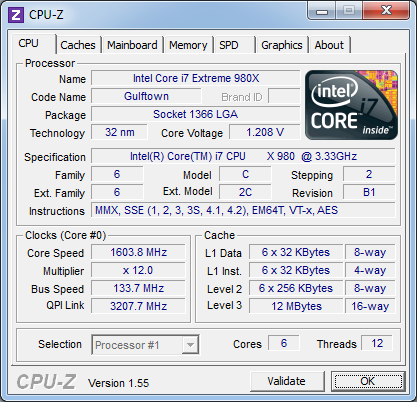
\includegraphics[scale=1]{imgs/cpu-z.png} 
\end{center}

%%%%%%%%%%%%%%%%%%%%%%%%%%%%%%%%%%%%%%%%%%%%%%%%%%%%%%%%%%%%%%%%

\newpage
\section{Трассировка лучей}
Классический ray tracing~[\cite{sivakov}], или метод трассировки лучей, предложен Артуром Аппелем (Arthur Appel) еще аж в 1968 году и дополнен алгоритмом общей рекурсии, разработанным Whitted в 1980 году. Понадобилось почти 12 лет эволюции вычислительных систем, прежде чем этот алгоритм стал доступен для широкого применения в практических приложениях. Реализация высокопроизводительной версии трассировки лучей уже предпринимаются различными компаниями. О сложности задачи трассировки лучей можно прочитать в соответствующих источниках~[\cite{biovulf}].

\subsection{Алгоритмы трассировки лучей}
Суть метода заключается в отслеживании траекторий лучей и расчета взаимодействий с лежащими на траекториях объектами, от момента испускания лучей источником света до момента попадания в камеру. Под взаимодействием луча с объектами понимаются процессы диффузного (в смысле модели локальной освещенности), многократного зеркального отражения от их поверхности и прохождение лучей сквозь прозрачные объекты. Таким образом, ray tracing – первый метод расчета глобального освещения, рассматривающий освещение, затенение (расчет тени), многократные отражения и преломления. Различают два основных вида метода трассировки лучей: \textbf{\textit{прямой}} -- \index{forward ray tracing}forward ray tracing, и \textbf{\textit{обратный}} -- \index{backward ray tracing}backward ray tracing.

\subsubsection{Прямой метод трассировки лучей}
В прямом методе траектории лучей строятся от источника ко всем точкам всех объектов сцены (первичные лучи). Затем проверяется ориентация каждой точки относительно источника, и, если она лежит на стороне объекта, обращенной в противоположную от источника сторону, точка из расчетов освещенности исключается. Для всех остальных точек вычисляется освещенность с помощью локальной модели освещения. Если объект не является отражающим или прозрачным, то есть поверхность объекта только диффузно рассеивает свет, траектория луча на этой точке обрывается (заканчивается). Если же поверхность объекта обладает свойством отражения (\index{reflection}reflection) и/или преломления (\index{refraction}refraction), из точки строятся новые лучи, направления которых совершенно точно определяются законами отражения и преломления.
\par
    Для построенных таким образом траекторий новых лучей может быть только три исхода. Луч либо выходит за пределы видимой из камеры области сцены, в этом случае все проделанные для него до этого момента расчеты освещенности отбрасываются, поскольку они не принимают участия в формировании изображения. Или луч попадает в камеру, тогда рассчитанная освещенность формирует цвет соответствующего пиксела изображения. Или луч встречает на своем пути новый
объект, тогда для новой точки пересечения повторяется расчет освещенности и построения лучей отражения и преломления в зависимости от свойств поверхности объекта (рекурсия). Построение новых траекторий и расчеты ведутся до тех пор, пока все лучи либо попадут в камеру, либо выйдут за пределы видимой области. Очевидно, что при прямой трассировке лучей мы вынуждены выполнять расчеты для лучей, которые не попадут в камеру, то есть, проделывать бесполезную работу. По некоторым оценочным данным доля таких "слепых"лучей довольно велика. Эта главная, хотя и далеко не единственная, причина того, что метод прямой трассировки лучей считается неэффективным и на практике не используется(в чистом виде).

\subsubsection{Обратный метод трассировки лучей}
Обратной метод трассировки лучей, или backward ray tracing. Этот метод расчетов основывается на построении лучей от наблюдателя через плоскость экрана вглубь сцены, а не от источника, то есть -- наоборот. Этот способ достаточно изящен, что позволяет решить массу проблем, возникающих при прямой трассировке, а сам метод отличается простотой и понятностью. Лучи теперь строятся иначе. А именно, по двум точкам: первая точка, общая для всех лучей – положение камеры (наблюдателя), вторая точка определяется положением пиксела на плоскости видового окна. Таким образом, направление каждого луча строго определено (две точки в пространстве определяют одну и только одну прямую – школьный курс геометрии), и количество первичных лучей также известно – это общее количество пикселей видового окна. Например, если видовое окно имеет 1920 пикселей по ширине и 1200 пикселей по высоте, количество лучей составит 1920 х 1200 = 2 304 000. Каждый луч
вдоль заданного направления продлевается от наблюдателя вглубь трехмерной сцены, и для каждой траектории выполняется проверка на пересечение со всеми объектами сцены и с отсекающими плоскостями. Если пересечений с объектами нет, а есть пересечение только с плоскостью отсечения, значит луч выходит за пределы видимой части сцены, и соответствующему пикселю видового окна присваивается цвет фона. Если луч пересекается с объектами сцены, то среди всех объектов выбирается тот, который ближе всего к наблюдателю. В точке пересечения с таким объектом строится три новых, так называемых вторичных луча. \par

\begin{center}
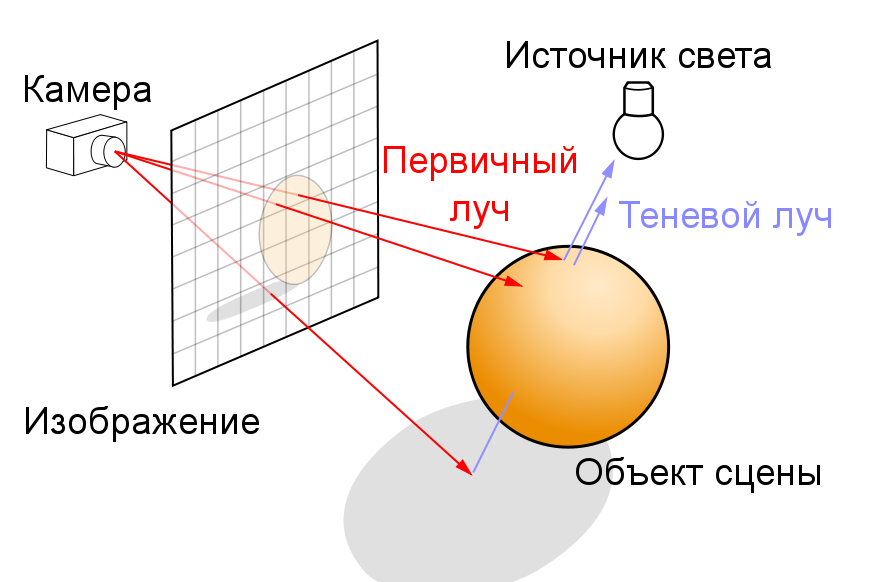
\includegraphics[scale=0.5]{imgs/Ray_trace_diagram_rus.png} 
\end{center}

Первый луч строится в направлении источника света. Если источников несколько, строится несколько таких лучей, по одному на каждый источник. Основное назначение этого луча – определить ориентацию точки (обращена точка к источнику или от него), наличие объектов, закрывающих точку от источника света, и расстояние до источника света. Если точка обращена в противоположную сторону от источника света или закрыта другим непрозрачным объектом, освещенность от такого источника не рассчитывается, точка находится в тени. В случае затеняющего прозрачного объекта интенсивность освещения уменьшается в соответствии со степенью прозрачности. Если точка закрыта от освещения всеми источниками сцены, ей присваивается фоновый (\index{ambient или фоновый цвет}ambient) цвет. В противном случае точка освещена, интенсивность и цвет освещения рассчитываются при помощи локальной модели освещенности, как сумма освещенностей от всех источников, для которых эта точка не закрыта другими объектами. Этот тип луча получил название \index{shadow ray или теневой луч} \textit{\textbf{shadow ray}} (иногда его еще называют \index{illumination ray}illumination ray) – теневой луч. Если поверхность объекта не является отражающей и непрозрачна, теневой луч – единственный тип лучей который строится, траектория первичного луча обрывается (заканчивается), и дальнейшие расчеты не выполняются. Рассчитанный цвет (освещенности или тени) присваивается тому пикселю видового окна, через который проходит соответствующий первичный луч.
   \par
   Второй луч строится, если поверхность объекта обладает отражающими свойствами, и называется \index{reflection ray или отраженный луч} reflection ray, или луч отражения. Направление отраженного луча определяется по закону:
$$
	\vec{R} = \vec{I} - 2 \cdot \vec{N} (\vec{N} , \vec{I})
$$
где $\vec{R}$ - отраженный луч, $\vec{I}$ - падающий пераичный луч, $\vec{N}$ - нормаль к поверхности в точке соударения.
Для отраженного луча проверяется возможность пересечения с другими объектами сцены. Если пересечений нет, то интенсивность и цвет отраженного луча равна интенсивности и цвету фона. Если пересечение есть, то в новой точке снова строится три типа лучей – теневые, отражения и преломления.
Третий луч строится, если поверхность объекта прозрачна, и носит название \index{transparency ray или преломленный луч}transparency ray, т. е. луч преломленный. Направление для преломленного луча определяется следующим образом:
$$
 \vec{T} = \frac{n_1}{n_2} \cdot \vec{I} - \left[ \cos \alpha + \frac{n_1}{n_2} \cdot \left(\vec{N},\vec{I} \ \right) \right] \cdot \vec{N}
$$
$$
\cos \alpha = \sqrt{1 - \left( \frac{n_1}{n_2} \right) ^2 \cdot \left(1-\left(\vec{N},\vec{I}\ \right)^2\right)}
$$
где $\vec{T}$ - переломленный луч, $n_1$ - коэффициент рефракции для первой среды ( в которой растространяется первичный луч ), $n_2$ - коэффициент рефракции для второй среды прозрачного объекта.

Так же, как и в предыдущем случае, проверяется пересечение вновь построенного луча с объектами, и, если они есть, в новой точке строятся три луча, если нет -- используется интенсивность и цвет фона.

Таким образом, для каждого первичного луча можно построить древовидную структуру. Если древовидная структура для данного луча построена, то расчет освещенности можно выполнить в следующем порядке. Для каждой ветви дерева спускаемся вдоль древовидной структуры к последнему пересечению вторичного луча и поверхности (будем дальше называть их узлами). Поскольку это последний узел в цепи, то  вкладов от преломлений и отражений нет, поэтому, освещенность узла вычисляется при помощи локальной модели освещения с учетом видимости источников света для данного узла. Затем, вычисленная освещенность передается вверх по ветви к следующему ближайшему узлу. Освещенность в этом узле будет вычисляться по формуле:

$$
 \vec{I}_{total} = \vec{I}_{local} + K_{reflection} \cdot \vec{I}_{reflection} + K_{refraction} \cdot \vec{I}_{refraction}
$$

где $\vec{I}_{total}$ - полная освещенность в точке, $\vec{I}_{local}$ - локальная освещенность в точке, вычисленная от источников освещения с помощью одной из локальной модели освещенности, $K_{reflection}$ - коэффициент, определяющий отражающие свойства поверхности, $\vec{I}_{reflection}$ - освещенность предыдущей точки, переданная вдоль ветки отражения,   $K_{refraction}$ - коэффициент, определяющий преломляющие свойства поверхности $\vec{I}_{refraction}$ - освещенность предыдущей точки, переданная вдоль ветки преломления

Естественным завершением трассировки лучей является выход всех испущенных вторичных лучей за пределы видимой области и их рассеяние на чисто диффузных объектах. Результат вычислений будет наиболее точным. Но, если сцена достаточно сложна, такой расчет будет очень медленным, а в некоторых случаях и невозможным по причине ограниченности аппаратных ресурсов. Легко увидеть, что вклад освещенности от каждого нового вторичного луча очень быстро уменьшается по той простой причине, что коэффициенты свойств отражения и преломления материалов меньше единицы. Поэтому часто трассировку лучей прекращают, когда вклад от следующего узла ветви становится меньше заданной величины. Это также достаточно точный метод расчетов, который может быть использован для получения качественных результатов при определенных условиях. Наконец, для получения оценочного расчета можно оборвать трассировку лучей после выполнения заданного количества итераций, это самый быстрый и наименее точный расчет.

\subsubsection{Достоинства и недостатки}

Основные достоинства рекурсивного метода обратной трассировки лучей – расчет теней, многократных отражений и преломлений, значительно повысивших степень реалистичности получаемых изображений.
Основные недостатки: неучет вторичного освещения от диффузно отраженного объектами света; низкая скорость и высокая вычислительная стоимость расчетов – в классическом рейтресинге необходимо проверять на пересечение каждый луч со всеми объектами сцены, в результате от 70 до 95 процентов всего времени расчетов тратится на вычисление пересечений; резкие границы цветовых переходов тени/подсветок/прозрачности; \index{aliasing}aliasing – "зазубренность" линий и т. д.; дискретность определяющих цвет пиксела первичных лучей – одного первичного луча недостаточно для корректного определения цвета пиксела, формирующего изображение.


\subsection{Модели освещения}

В соответствии с принятым в компьютерной графике подходом, расчет освещенности распадается на две основные задачи. Первая – определить способ расчета освещенности в произвольной точке трехмерного пространства, решается при помощи построения обобщенной математической модели освещенности (Illuminating model). Вторая задача – применение Illuminating model для компьютерных расчетов освещенности трехмерных объектов с конкретной геометрией и свойствами поверхности, решается при помощи так называемой модели затенения (Shading model).

Моделей освещенности к настоящему моменту разработано несколько. Самая первая,и самая простая – локальная модель освещенности. Эта модель не рассматривает процессы светового взаимодействия объектов сцены между собой, а только расчет освещенности самих объектов. Вторая, глобальная модель освещенности – Global Illuminations, рассматривает трехмерную сцену как единую систему и пытается описывать освещение с учетом взаимного влияния объектов. В рамках этой модели рассматриваются такие вопросы, как многократное отражение и преломление света (ray tracing), рассеянное освещение (radiosity), каустик(caustic) и фотонные карты (photon mapping) и другие. 

\subsubsection{Глобальные модели освещения}

Глобальное освещение (global illumination) — это название ряда алгоритмов, используемых в 3D-графике, которые предназначены для добавления более реалистичного освещения в трёхмерные сцены. Такие алгоритмы учитывают не только свет, который поступает непосредственно от источника света (прямое освещение, англ. direct illumination), но и такие случаи, в которых лучи света от одного и того же источника, отражаются на других поверхностях сцены (непрямая освещенность, англ. indirect illumination).

Теоретически отражение, преломление, тень — примеры глобального освещения, потому что, для их имитации необходимо учитывать влияние одного объекта на другие (в отличие от случая когда на объект падает прямой свет). На практике, однако, только моделирование диффузного отражения или каустики называется глобальным освещением.

Изображения полученные в результате применения алгоритмов глобального освещения часто кажутся более фотореалистичными, чем те, в процессе рендеринга которых применялись алгоритмы только прямого освещения, но для просчета глобального освещения требуется гораздо больше времени.

\subsubsection{Локальные модели освещения}

Существующие локальные модели освещения можно разделить на две категории. К первой категории относятся эмпирические модели. Они обычно эффективны в плане быстродействия и некоторые из них дают довольно реалистичную картинку. Они обычно не оперируют такими физическими величинами, как световая энергия, или световой поток. Однако эти модели находят довольно широкое применение в областях, где не требуется точная физическая информация об освещении (например, спецэффекты в фильмах, программы для художников и дизайнеров, для рекламных целей)

Ко второй категории относятся модели, базирующиеся на физических представлениях о теории света. Изображения, полученные с использованием этих моделей, очень хорошо соотносятся с экспериментальными данными. Поэтому эти модели находят применение там, где важна точная имитация поведения света (оформление интерьеров, архитектура)

\subsubsection{Модель Фонга}

Это эмпирическая модель. В самом общем случае, в свете требования фотореалистичности, эта модель учитывает и неявное ambient-освещение. Ambient-освещение, или его еще называют фоновым (background), – это окружающее объект освещение от удаленных источников, чье положение и характеристики не известны. Необходимость учета ambient-освещения, пусть и очень грубо, обусловлена тем, что его вклад может быть достаточно велик – до 50\% от общей освещенности. В Local Illumination считают, что фоновое освещение задает цвет (и его интенсивность) объекта в отсутствии явных источников света или в тени. Не несет никакой информации об объекте, кроме значения простого цвета, равномерно заливающего контур объекта.

Интенсивность такого освещения постоянна и равномерно распределена во всем пространстве, расчет его отражения поверхностью выполняется по формуле:

$$
 \vec{I}_{amb} = K_{a} \cdot \vec{I}_{a}
$$

где $\vec{I}_{amb}$  - интенсивность отраженного ambient освещения, $K_{a}$ - коэффициент, характеризующий отражающие свойства поверхности для  ambient-освещения, $\vec{I}_{a}$ - исходная интенсивность ambient-света, падающего на поверхность.

Часть света от прямых источников зеркально отражается поверхностью, а остальной свет диффузно рассеивается во всех направлениях. Кроме чисто зеркального отражения, которое имеют идеально отполированные поверхности, различают так называемое glossiness или распределенное зеркальное отражение – отражение в некотором створе углов, а не на один единственный угол. Такое рассеяние света обусловлено микрорельефом ("шероховатостью") поверхности, то есть поверхность реальных объектов не является идеально гладкой, а состоит из большого количества микровыступов и впадин, которые зеркально отражают падающий свет под разными углами. Результатом glossy-отражения является specular highlight – яркий световой блик, имеющий размер в зависимости от степени шероховатости поверхности. 

Интенсивность рассеянного света зависит от угла падающего на поверхность света по закону Ламберта (Lambert):

$$
 \vec{I}_{diff} = K_{diff} \cdot \vec{I}_{d} \cdot \cos(\alpha)
$$
 
где $\vec{I}_{d}$ - интенсивность падающего на поверхность света, $K_{diff}$ - коэффициент, характеризующий рассеивающие свойства поверхности, $\cos(\alpha)$ - угол между направлением на источник света и нормалью поверхности

Другими словами, поверхность будет освещена больше, если свет падает на нее перпендикулярно ($\alpha = 0$), и меньше, если свет падает под любым другим углом, поскольку в этом случае увеличивается освещаемая площадь. Диффузно рассеянный свет является главным источником визуальной информации о геометрии трехмерных объектов.

Как было уже сказано ранее, свет отражается зеркально в некотором створе углов, и для большинства реальных материалов мы всегда видим зеркальную подсветку в форме светового пятна, а не в форме яркой точки. Поэтому, для расчета интенсивности зеркально отраженного света используется формула, предложенная Фонгом:

$$
 \vec{I}_{spec} = K_{spec} \cdot \vec{I}_{s} \cdot \cos^n(\beta)
$$

где $\vec{I}_{spec}$ - интенсивность зеркально отраженного света,  $\vec{I}_{s}$ - интенсивность источника света,  $\vec{K}_{s}$ - коэффициент, характеризующий свойства зеркального отражения поверхности
$\beta$ - угол между направлением идеального отражения и направлением на наблюдателя, степень $n$ определяет размер пятна светового блика, чем больше $n$, тем меньше световой блик, и тем ближе отражающие свойства поверхности к свойствам идеального зеркала.

Формула Фонга – пример компьютерной фикции, поскольку она не имеет физического смысла. Ее используют просто потому, что она дает хорошие практические результаты. 

Таким образом, локальная модель освещенности предполагает расчет отраженной фоновой освещенности, диффузного и зеркального отражения от прямых источников: 

$$
 \vec{I}_{local} =  K_{amb} \cdot \vec{I}_{amb} +  K_{diff} \cdot \vec{I}_{diff} \cdot \left( \vec{L},\vec{N} \right) + K_{spec} \cdot \vec{I}_{spec} \cdot \left( \vec{R},\vec{V} \right)^n
$$



\subsection{Примитивы}
\subsubsection{\index{Плоскость}Плоскость}
Для определения пресечения луча с плоскостью, необходимо найти точку в пространстве, которая будет удовлетворять двум уравнениям: уравнению луча и уравнению плоскости.
\par
Уравнение луча:
\begin{equation}
\left\{
\begin{array}{ccccc}
x & = & x_0 & + & t \cdot x_d \\
y & = & y_0 & + & t \cdot y_d \\
z & = & z_0 & + & t \cdot z_d \\
\end{array}
\right.
\label{equation_ray}
\end{equation}
или
$$
\vec{R}(t) = \vec{O} + t \cdot \vec{D}
$$
где $O = \VECXYZ{0} $ - начало луча, а $D = \VECXYZ{d} $ - направление луча. 
\par
Уравнение плоскости задается следующим образом:
\begin{equation}
Ax + By + Cz + D = 0
\label{equation_plane}
\end{equation}
\par
Для того, что бы найти точку пересечения луча с плоскостью, необходимо подставить уравнение (\ref{equation_ray}) в (\ref{equation_plane}):
$$
A(x_0 + t \cdot x_d) + B(y_0 + t \cdot y_d) + C(z_0 + t \cdot z_d) + D = 0
$$
Раскроем скобки и приведем подобные
$$
t(Ax_d + By_d + Cz_d ) + Ax_0 + By_0 + Cz_0 + D = 0
$$
найдем неизвестную величину t
$$
 t = - \frac{Ax_0 + By_0 + Cz_0 + D}{Ax_d + By_d + Cz_d}
$$
из уравнения видно, что луч либо пересекает плоскость в какой то точке, либо нет. Это связано с тем, что если $Ax_d + By_d + Cz_d = 0$, то плоскость и луч параллельны друг другу. Т.к. $P = \VEC{A}{B}{C} $ - это нормаль к поверхности, то из геометрии известно, что если $( D , P ) = 0$, то вектора параллельны.
\par
   Для того, что бы найти величину $t$, необходимо рассчитать всего несколько скалярных произведений:
$$
t = - \frac{(O, P) + D}{(D, P)}
$$
при условии, что $(D, P) \neq 0$

\subsubsection{\index{Сфера}Сфера}
Для сферы необходимо проделать те же выкладки.
Уравнение луча:
\begin{equation}
\left\{
\begin{array}{ccccc}
x & = & x_0 & + & t \cdot x_d \\
y & = & y_0 & + & t \cdot y_d \\
z & = & z_0 & + & t \cdot z_d \\
\end{array}
\right.
\label{equation_ray}
\end{equation}
или
$$
\vec{R}(t) = \vec{O} + t \cdot \vec{D}
$$
Уравнение сферы записывается следующем образом:
\begin{equation}
(x-x_c)^2 + (y-y_c)^2 + (z-z_c)^2 = r^2
\label{equation_sphere}
\end{equation}
где $S = \VECXYZ{c}$ - центр сферы, а $r$ - радиус. Подставим уравнение (\ref{equation_ray}) в (\ref{equation_sphere}):
$$
\left( (x_0 + t \cdot x_d) - x_c \right)^2 + 
\left( (y_0 + t \cdot y_d) - y_c \right)^2 + 
\left( (z_0 + t \cdot z_d) - z_c \right)^2 = r^2
$$
приведем это уравнение в виду
\begin{equation}
A \cdot t^2 + B \cdot t + C = 0
\label{equation_square}
\end{equation}
после раскрытия скобок и приведения подобных, получаем:
\par
$$
A = x^2_d + y^2_d + z^2_d
$$ 
\par
$$
B = 2x_d(x_0 - x_c) + 2y_d(y_0 - y_c)  + 2z_d(z_0 - z_c) 
$$ 
\par
$$
C = (x_0 - x_c)^2 + (y_0 - y_c)^2 + (z_0 - z_c)^2 
$$
Если уравнение (\ref{equation_square}) не имеет вещественных решений, то луч не пересекает сферу. Если имеется два решения, то наименьший положительный корень этого уравнения определит на луче ближайшую точку пересечения луча со сферой.
\par
Рассмотрим подробнее как вычисляются коэффициенты $A$, $B$, $C$:
\par
$$
A = x^2_d + y^2_d + z^2_d = (D, D)
$$ 
\par
$$
B = 2x_d(x_0 - x_c) + 2y_d(y_0 - y_c)  + 2z_d(z_0 - z_c)  = 2 \cdot (D, D - S)
$$ 
\par
$$
C = (x_0 - x_c)^2 + (y_0 - y_c)^2 + (z_0 - z_c)^2 = (O - S, O - S )
$$
Далее решаем обыкновенное квадратное уравнение и находим корни и получаем значение $t$
$$
t_{1,2} = \frac{-B \pm \sqrt{B^2 - 4 \cdot A \cdot C}}{2 \cdot A}
$$

$$
t_{1} = \frac{ - 2 \cdot (\vec{D}, \vec{D} - \vec{S}) + \sqrt{(2 \cdot (\vec{D}, \vec{D} - \vec{S}))^2 - 4 \cdot (\vec{D}, \vec{D}) \cdot (\vec{O} - \vec{S}, \vec{O} - \vec{S} )}}{2 \cdot (\vec{D}, \vec{D})}
$$

$$
t_{2} = \frac{ - 2 \cdot (\vec{D}, \vec{D} - \vec{S}) - \sqrt{(2 \cdot (\vec{D}, \vec{D} - \vec{S}))^2 - 4 \cdot (\vec{D}, \vec{D}) \cdot (\vec{O} - \vec{S}, \vec{O} - \vec{S} )}}{2 \cdot (\vec{D}, \vec{D})}
$$

\subsubsection{\index{Треугольник}Треугольник}
Алгоритм пересечения луча и треугольника основан на барицентрических координатах.
\par
Барицентрические координаты -- координаты точки $n$-мерного аффинного пространства $A^n$, отнесенные к некоторой фиксированной системе из $(n + 1)$-ой точки $p_0, p_1, \dots, p_n$ , не лежащих в $(n -1)$-мерном подпространстве. Пусть $z$ есть произвольная точка в $A^n$. Каждая точка $x \in A^n$ может быть единственным образом представлена в виде суммы
$$
	x = z + \alpha_1 \cdot z\vec{p_1} + \alpha_2 \cdot z\vec{p_2} + \cdots + \alpha_n \cdot z\vec{p_n} 
$$
где $\alpha_1, \alpha_2, \dots,  \alpha_n $ вещественные числа, удовлетворяющие условию
$$
\alpha_1 + \alpha_2 + \cdots + \alpha_n  = 1
$$
Числа $\alpha_1, \alpha_2, \dots,  \alpha_n $ называются барицентрическими координатами точки $x$. Легко видеть, что барицентрические координаты не зависят от выбора $z$.

Точка $T(u,v)$, принадлежащая треугольнику, может быть записана в виде:
\begin{equation}
\label{triangle_bar}
T(u,v) = (1-u-v)V_0 + uV_1 + vV_2
\end{equation}

\noindent где $(u,v)$ -- это бариецентрические координаты такие, что $u \geq 0$, $v \geq 0$ и $u + v \leq 1$

Вычисление пересечения между лучем(\ref{equation_ray}) и треугольником(\ref{triangle_bar}), это решение следующего уравнения:

$$
O + tD = (1-u-v)V_0 + uV_1 + vV_2
$$

\noindent после нескольких очевидных преобразований:

$$
O + tD = V_0 - uV_0 - vV_0 + uV_1 + vV_2
$$
$$
O - V_0 = - tD + uV_1 - uV_0 + vV_2 - vV_0
$$

$$
- tD + u(V_1 - V_0) + v(V_2 - V_0) = O - V_0
$$

\noindent получаем:

\begin{equation}
\label{ray_cross_tr}
\left[ -D, V_1 - V_0 , V_2 - V_0\right] 
\left[  
\begin{array}{c} t \\ u \\ v \\ \end{array}
\right] = O - V_0
\end{equation}

Что бы решить задачу, необходимо найти вектор $\VEC{t}{u}{v}$. Обозначив $E_1 = V_1 - V_0$, $E_2 = V_2 - V_0$ и $T = O - V_0$ решим уравнение (\ref{ray_cross_tr}), используя метод Крамера:

\begin{equation}
\label{ray_cross_tr_solv}
\left[  
\begin{array}{c} t \\ u \\ v \\ \end{array}
\right] = 
\frac{1}{| -D , E_1, E_2|} 
\left[  
	\begin{array}{lcccl}
	|& T , & E_1, &E_2 & | \\
	|&-D , & T  , &E_2 & | \\
	|&-D , & E_1, &T   & | \\
	\end{array}
\right] 
\end{equation}

\noindent Из курса линейной алгебры известно, что: $|A, B, C| = - (A \times C) \cdot B = - (C \times B) \cdot A$. Принимая во внимания этот факт, перепишем уравление (\ref{ray_cross_tr_solv}).

\begin{equation}
\label{ray_cross_tr_solv2}
\left[  
\begin{array}{c} t \\ u \\ v \\ \end{array}
\right] = 
\frac{1}{(D \times E_2)\cdot E_1} 
\left[  
	\begin{array}{c}
	(T \times E_1) \cdot E_2 \\
	(D \times E_2) \cdot T \\
	(T \times E_1) \cdot D \\
	\end{array}
\right] = 
\frac{1}{P \cdot E_1} 
\left[  
	\begin{array}{c}
	Q \cdot E_2 \\
	P \cdot T \\	
	Q \cdot D \\	
	\end{array}
\right]
\end{equation}
где $P = (D \times E_2)$ и $Q = T \times E_1$


%%%%%%%%%%%%%%%%%%%%%%%%%%%%%%%%%%%%%%%%%%%%%%%%%%%%%%%%%%%%%%%%%%%%%%%%%%%%%%%%%%%%%%%%%%%

\newpage
\section{Оптимизация}
Оптимизация -- как способ программирования по уровням архитектуры сверху вниз.

\subsection{Шаблоны C++}

\subsubsection{Понятие шаблона}

Шаблоны(Templates) были введены в язык C++ как средство, позволяющие параметризовать типы данных. Это связано с тем, что для классов или функций приходилось реализовывать одни и те же алгоритмы, но для разных типов данных. Получали дублирование кода, и тем самым росло число ошибок. 
Пример. Реализовать функцию, которая возвращает максимальное значение из 2 чисел.

\cppsource{src/deftemplate.tex}{Несколько реализация функции {\bf max}}

\noindent
и так далее. Приходится писать один и тот же код несколько раз. Во второй функции можно было допустить ошибку (например указать неправильный знак сравнения), которую потом очень трудно найти. Или наоборот, после обнаружения ошибки, придется править код во всех реализациях функции max (возможна ситуация, когда в нескольких местах ошибка была исправлена, а в остальных пропущена или забыта). С этими проблемами помогли справится шаблоны, которые параметризовали типы данных следующим образом:

\cppsource{src/definetemplate.tex}{Шаблонное определение функции {\bf max}}

%\noindent
Т. о. работу которую выполнял программист теперь выполняет компилятор. При вызове функции, в качестве параметров которых нужно сравнить два int, компилятор сам из шаблона выведет функцию max(int,int).
\subsubsection{Вычисление на шаблонах}
Сегодня шаблоны используют различным образом, не так как ожидали изобретатели
шаблонов С++. Сегодня программирование на шаблонах включают различные техники, такие как: обобщенное программирование, вычисление во время компиляции, шаблонные выражения(expression templates), мета-программирование, и др.

\noindent Рассмотрим пример вычисления факториала. \\
\noindent Факториал числа N это: $N! = N \cdot (N-1) \cdot \dots \cdot 1$

Рекурсивная реализация факториала, без использование шаблонов, приведена в следующем листинге:

\cppsource{src/rekfactorial.tex}{Рекурсивная реализация факториала}

Эту функцию следует использовать следующим образом:
\begin{verbatim}
cout << factorial(7) << endl;
\end{verbatim}
Вызывать рекурсивно функцию - это очень большие накладные расходы. Несмотря на то, что мы указало компилятору встроить функцию (inline), компилятор проигнорирует это, так как он не может сделать постановку в рекурсию. Можно добиться большего успеха, если реализовывать это, как класс с шаблоном.

\cppsource{src/templatefactorial.tex}{Реализация факториала на шаблонах}

Можно заметить, что у данного шаблона нет ни данных, ни функциональных участков, это только определение перечислимого типа. Для того чтобы можно было определить шаблон для n, нужно для начала определить шаблон для n-1, т. е. для n-2, n-3 и т. д. В итоге получаем рекурсию. Следует заметить, что в качестве параметра шаблона используется обычный тип int. По стандарту, в качестве параметров шаблона могут быть использованы только перечислимые типы. В нашем случае есть параметр шаблона типа int, это означает, что в этот шаблон будет подставлено постоянное число типа int. Что бы воспользоваться данным классом необходимо написать следующие:
\begin{verbatim}
cout << factorial<7>::ret << endl;
\end{verbatim}
Компилятор рекурсивно определяет значение факториала<7>, затем <6> и так далее. Так как это рекурсия, то что бы не зациклится необходимо вовремя остановится. Любая рекурсия нуждается в остановки, и это не исключение. Это можно сделать с помощью специализации шаблона(т.е. определение для частного случая).

\cppsource{src/specfactorial.tex}{Специализация шаблона вычисления факториала}

Когда компилятор начнет определять специализацию для <0>, то он подставит имеено эту реализацию и рекурсия завершится. В результате, получится следующая структура:

\cppsource{src/finfactorial.tex}{Развернутая структура вычисления факториала}

Как видно из примера, от структуры уже ничего ни осталось и при уровне оптимизации начиная с O1, компилятор подсчитает выражение и вместо:
\begin{verbatim}
cout << factorial<7>::ret << endl;
\end{verbatim}
Подставит, подсчитанное выражение:
\begin{verbatim}
cout << 5040 << endl;
\end{verbatim}
Проверить это можно дизассемблировав данный пример и увидеть в коде число 5040.

\subsection{SIMD инструкции}
Применение SIMD инструкций в классе vec4.

\subsection{Ускоряющие структуры}
BVH. Алгоритмы построения и поиска.

%%%%%%%%%%%%%%%%%%%%%%%%%%%%%%%%%%%%%%%%%%%%%%%%%%%%%%%%%%%%%%%%%%%%%%%%%%%%%%%%%%%%%%%%%%%

\newpage
\section{Постановка и результаты экспериментов}

Эксперименты проводилимь на 6 ядерном компьютере с процессором Intel Core i7 980x с частотой 3.33GHz, оперативной памятью 12 Гб, ОС - Calculate Linux 11.0 x64. 

Для сборки приложения с библиотекой tbb, необходимо, что бы компилятор поддерживал лямбда выражения из нового стандарта c++0x. На данный момент, этот стандарт поддерживает компилятор GCC 4.5.2

\subsection{Timer}
Для того, чтобы точно оценивать время работы каждого из алгоритмов, очень важно иметь такой инструмент как таймер, способный оценить время работы алгоритма. 
Проблема в том, что стандарные методы операционных систем не работают с нужной точностью. Когда идет речь о том, чтобы оценить время, который должен исполнятся очень много миллионов раз в секунду, важен каждый такт процессора и точность в миллисекунду и уж тем более в секундах просто неприемлема.

Для очень точной оценки времени работы алгоритмов, был специально написан высокоточный таймер на языке c++, с использованием ассемблера (AT\&T - синтаксиса).
Таймер выдает время в тактах процессора и включает в себя разные режимы подсчета времени.

\subsubsection{Алгоритм работы высокоточного таймера}

\cppsource{src/timer.tex}{Метод Start() и Stop() класса Timer}


\subsubsection{Эксперименты с высокоточным таймером}

\subsection{Вектора и Expression templates}

\subsection{Тестовая сцена}

\subsection{Эффективность расспаралеливания}

\subsection{TBB vs OpenMP}

\subsection{Влияние SIMD инструкций на скорость работы}

\subsection{Компилирование высокоуровнего кода в ассемблер}

Ассемблерные вставки, которые показывают что вычисление отражающего луча это одно SSE.

%%%%%%%%%%%%%%%%%%%%%%%%%%%%%%%%%%%%%%%%%%%%%%%%%%%%%%%%%%%%%%%%%%%%%%%%%%%%%%%%%%%%%%%%%%%

\newpage
\section*{Заключение}
\addcontentsline{toc}{section}{Заключение} 
Задача трассировки лучей является по настоящему трудным испытанием для центрального процессора. Несмотря на то, что процессор обладает хорошей производительностью на ядро, общей производительности ему не хватает. Несмотря на столь малые мощности, удалось реализовать достаточно быстрый алгоритм на центральном процессоре. Для большей производительности была разработана эффективная параллельная версия программы с использованием библиотеки TBB и
стандарта параллельного OpenMP. Благодаря использованию языка с++ и технику шаблонных выражений, удалось еще повысить производительность программы. Программа продемонстрировала хорошую производительность: используя всего лишь один процессор можно получать изображения в реальном времени.

%%%%%%%%%%%%%%%%%%%%%%%%%%%%%%%%%%%%%%%%%%%%%%%%%%%%%%%%%%%%%%%%%%%%%%%%%%%%%%%%%%%%%%%%%%%

\newpage
\begin{thebibliography}{99}
	\bibitem{morozov_kazan} Морозов А. С. Трассировка лучей в реальном времени на многоядерном процессоре. Высокопроизводительные параллельные вычисления на кластерных системах (HPC-2008). Материалы Восьмой Международной конференции-семинара. Казань, ноябрь 17-19, 2008. Труды конференции — Казань: Изд. КГТУ, 2008. - С. 241.
	\bibitem{morozov_microsoft} Морозов А. С. Высокопроизводительная реализация трассировки лучей с использованием Microsoft MPI. Технологии Microsoft в теории и практике программирования. Материалы конференции /Под ред. Проф. В.П. Гергеля. - Нижний Новгород: Изд-во Нижегородского госуниверситета, 2009. - 527 с.
	\bibitem{morozov_pavt} Морозов А. С. Сравнительный анализ алгоритма трассировки лучей на системах с общей и разделяемой памятью. Параллельные вычислительные технологии (ПаВТ’2009): Труды международной научной конференции (Нижний Новгород, 30 марта - 3 апреля 2009 г.). - Челябинск: Изд. ЮурГУ, 2009. - 839 с
	\bibitem{latex} Львовский С.М. Набор и верстка в системе \LaTeX. – 4-е изд., стереотипн. – М.: МЦНМО, 2006
	\bibitem{alloftex} Кнут, Дональд, Э. Все про \TeX. : Пер. с англ. --- М. : Издательский дом ''Вильямс'', 2003. --- 560 с. : ил. --- Парал. Тит. англ.
	\bibitem{inteloptimize} Гербер Р., Бик А., Смит К., Тиан К. Оптимизация ПО. Сборник рецептов. --- СПб.: Питер, 2010. --- 352 с.: ил. --- (Серия ''Библиотека программиста'').
	\bibitem{templatecpp} Вандевурд, Дэвид, Джосаттис, Николаи М. Шаблоны C++: справочник разработчика. : Пер. с англ. --- М. : Издательский дом ''Вильямс'', 2008. --- 544 с. : ил. --- парал. тит. англ.
	\bibitem{straustrupcpp} Б. Страуструп Язык программирования C++. Специальное издание / Пер. с англ. --- М.: ООО ''Бином-Пресс'', 2006. --- 1104 с.: ил.
	\bibitem{sivakov} Сиваков И. Как компьютер рассчитывает изображения. Технология программного рендеринга, 11.03.2004. \\ (\href{http://www.fcenter.ru/online.shtml?articles/hardware/videos/8749}{http://www.fcenter.ru/online.shtml?articles/hardware/videos/8749})
	\bibitem{biovulf} Дмитрий Мороз. "Беовульф": Создание фильма, 11.12.2007.\\ (\href{http://www.3dnews.ru/editorial/beowulf}{http://www.3dnews.ru/editorial/beowulf})
	\bibitem{intelintrinsic} Intel® C++ Intrinsics Reference \\ (\href{http://www.intel.com/products/processor/manuals/}{http://www.intel.com/products/processor/manuals/})
	\bibitem{intelmanual} Intel 64 and IA-32.Architectures Software Developer's Manual \\ (\href{http://www.intel.com/products/processor/manuals/}{http://www.intel.com/products/processor/manuals/})
	\bibitem{tbbtutor} Intel® Threading Building Blocks. Tutorial \\ (\href{http://www.threadingbuildingblocks.org/}{http://www.threadingbuildingblocks.org/})
	\bibitem{tbbmanual} Intel® Threading Building Blocks. Reference Manual \\ (\href{http://www.threadingbuildingblocks.org/}{http://www.threadingbuildingblocks.org/})
	\bibitem{cppexpressiontemplate} C++ Expression Templates An Introduction to the Principles of Expression Templates, 2003 \\ (\href{http://www.angelikalanger.com/Articles/Cuj/ExpressionTemplates/ExpressionTemplates.htm}{http://www.angelikalanger.com/.../ExpressionTemplates.htm})
	\bibitem{intelcore980x} Шесть ядер для десктопа: Intel Core i7-980X Extreme Edition, 07.04.2010 \\ (\href{http://www.fcenter.ru/online.shtml?articles/hardware/processors/28480}{http://www.fcenter.ru/online.shtml?articles/hardware/processors/28480})
	\bibitem{rdtscp} How to Benchmark Code Execution Times on Intel IA-32 and IA-64 Instruction Set Architectures. September 2010
\end{thebibliography}

\newpage
\input{rt2cpu.ind}

\end{document}


\end{document}


\end{document}


\end{document}
